%第二章
\chapter{AUV设计}

\section{推进器布置}

\subsection{推进器的布置形式对机敏性的影响}

水下机器人所使用的推进器有多种类型,每种都有其特点和应用场景。以下是几种常见的推进器类型及其特点:

\textbf{可旋转方向推进器:}这种推进器能够围绕固定的轴(通常是{\bf{Z}}轴)旋转,从而能够在水下机器人的{\bf{X-Y}}平面上产生不同方向的推力。
这种设计的优势在于灵活性高,能够减少系统的总体能耗,并适应更广泛的任务需求。
然而,它的机械结构较为复杂,这也增加了控制系统的设计难度。

\textbf{固定式推进器:}这类推进器的中轴线相对于水下机器人的本体有一个固定的夹角,
这意味着一旦安装完毕,其推力方向就确定不变了。
固定式推进器简单可靠,虽然由于缺乏旋转能力,它们无法根据任务需求灵活调整推力方向,但是可以通过矢量合成来达到我们所想要的矢量方向。
本论文里涉及的推进器就是这种类型。

\textbf{槽道推进器:}这种推进器安装在水下机器人的壳体内部通道中,可以实现正向和反向旋转,
从而产生所需的推力。它们通常用于那些对外形设计有特殊要求的水下机器人,比如需要流线型设计以减少阻力的情况。

\textbf{控制面:}类似于飞机上的舵片,水下机器人也可以使用控制面来改变其姿态。这些控制面可以固定在不同位置,
以产生升力和阻尼力,帮助机器人进行俯仰和偏航等运动。它们的作用类似于鱼的鳍,能够辅助推进器完成复杂的三维运动。

在我们选择推进器的时候,螺旋桨推进器的叶片有顺时针跟逆时针,这两种推进器成对使用并且对称分布,以便能够抵消推进器工作时产生的扭矩。
根据我们需要的水下机器人的自由度,我们确定使用推进器的数量,选择的推进器的数量是要大于或者等于我们需要的水下机器人自由度。例如假如
我们想要水系机器人有六个自由度的运动,我们可以选择八个推进器。
在确定了推进器的数量之后,我们就要考虑推进器的布置,首先我们确定{\bf{X-Y}}平面上的推进器布置,我们以其中的一个推进器布置为例(如\autoref{fig:2-1}所示),其余的推进器布置可通过成对和对称来实现。

\begin{figure}[H]%H强制浮动体放置在其在源代码中出现的位置
    \centering
    \subfigure[{\fangsong }] {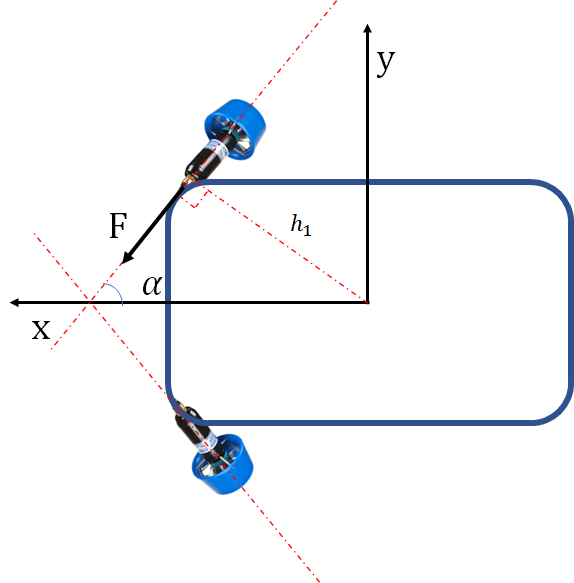
\includegraphics[width=7.25cm,height = 6.5cm]{毕设图片/2-1-1.png}}%
    \subfigure[{\fangsong }] {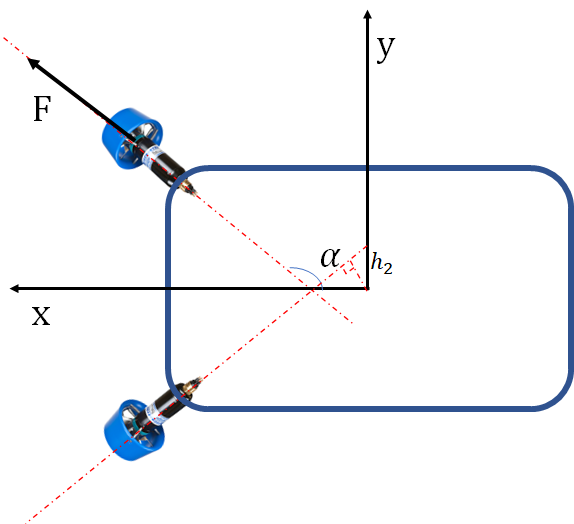
\includegraphics[width=7.25cm,height = 6.5cm]{毕设图片/2-1-2.png}}
    \caption{\label{fig:2-1}推进器布置示意图}
\end{figure}

当推进器的推力确定的时候,我们来确定\autoref{fig:2-1}中,$a$,$b$两种方式的优劣。其中$h_1$,$h_2$是力到轴$Z$的距离,有理论力学的基本理论
可以得到力对轴的矩的大小关系:
\begin{equation}
    \label{equ:2-1}
    F*h_1 > F*h_2
\end{equation}
力对轴的矩是产生旋转的原因,因此力对轴的矩的大小,跟水下机器人偏航运动的敏捷密切相关,力对轴的矩越大,旋转的角加速度会越大,机器人运动更加迅捷。
总的来说,$a$布局与$b$相比主要有以下几点优点:
\begin{enumerate}
    \item  推进器的性能有限,意味着当推力达到极致时,$a$布局方式会产生更大的角加速度,使得水下机器人运动更加的迅速。
    \item  当我们想要水下机器人以固定角加速度进行偏航运动时,意味着使用更小的推力就可以达到我们需要的角加速度,这使得推进器消耗的能量更小,使得水下机器人续航更长。
    \item  推进器在推力的范围内,能控制的角加速度范围变大,意味着控制更加敏捷,对水下机器人的控制量更加敏捷。
\end{enumerate}
\subsection{最优化建模}
确定了布局方式之后,我们就要确定\autoref{fig:2-1}中,$a$布局方式中 $\alpha $的大小。
确定 $\alpha $要考虑的因素,首先{\bf{X-Y}}平面的推进器跟水下机器人三个方向的自由度有关,分别是纵荡、横荡、偏航。估计三个方向上水下机器人在每次任务上行走距离的占比或者
运动时间的占比。因为我们主要是设计出机敏性更将强的水下机器人,我们还需要重点考虑三个方向上的加速能力,即加速度。
根据这些因素我们可以通过最优化求解的方式来求的最优的$\alpha $。
设我们想要的三个方向的占比分别为$a:b:c$,其中$  a+b+c = 1$。那么我们根据几何关系可以得到关于$\alpha $的函数解析式:

\begin{equation}
    \label{equ:2-2}
    f(\alpha) = aFcos(\alpha)+bFsin(\alpha)+cFh_1
\end{equation}


\begin{equation}
    \label{equ:2-3}
    h_1 = Lsin(\alpha)-Wcos(\alpha)
\end{equation}
其中,$\alpha$为力$F$与$X$轴的夹角,如\autoref{fig:2-1}中(a)所示;$L$是力作用点到$Y$轴的距离,$W$是力的作用点到$X$轴的距离。

对问题进行建模,并转化为标准形式可以得到:
\begin{equation}
    \begin{split}
    \label{equ:2-4}
    \underset{\alpha}{\min}  J = -f(\alpha)
    \\ s.t.
    \begin{cases}&F\cos(\alpha)-m{\alpha}_x\geq0 \\&F\sin(\alpha)-m{\alpha}_y \geq0\\&Fh_1-I{\alpha}_z\geq0\\&\alpha\geq0\\&\frac{\pi}{2}-\alpha\geq0\\&F-F_{min}\geq0
        \end{cases}
    \end{split}
\end{equation}
其中${\alpha}_x,{\alpha}_y$和${\alpha}_z$分别是$X,Y$方向的最小加速度与绕$Z$轴的最低角加速度,$F_{min}$是水下机器人工作的最小推力。
\subsection{最优化求解}

暂定SQP,C++,QT做一个交互界面。

\subsection{推力控制向量}

一般情况下,我们设计好推机器布置之后,就要根据我们的需求进行推力分配,传统的推力分配,是通过先求每个自由度方向所需的力或力矩,然后在通过求解布置矩阵的伪逆矩阵
来求解每个推进器上应该输出的推力。然而,对于每个控制问题而言,并不是每个推进器都是最佳的选择,例如当我们控制水下机器人水平前行的时候,并不需要垂直推进器的作用。
有时候我们又需要根据水下机器人的功能,来去修改推进器的布置形式,这个时候计算的布置矩阵就会因为某个推进器的整体变化而受到影响。特别的,当水下机器人执行任务的过程中
,出现某个推进器损坏或者不工作的情况时,如若改变推进器的布置矩阵,这将不利于系统的稳定。然而通过控制向量的方式对推进器进行增删操作,并不会对系统的布置矩阵产生
影响,有利于系统的稳定,极大的提高了水下机器人在水中遇到突发情况时的机敏性。推力控制向量如\autoref{equ:2-5}所示:
\begin{equation}
    \label{equ:2-5}
    {\beta}_i =  \left[ {\begin{array}{*{20}{c}}
        {f_1}\\
        {f_2}\\
        f_3\\
        f_4\\
        f_5\\
        f_6
        \end{array}} \right]
\end{equation}
其中,$i$ 表示第 $i$ 个推进器。  ${f_1}$表示推进器的纵荡系数,
${f_2}$表示推进器的横荡系数,
$f_3$表示推进器的垂荡系数,
$f_4$表示推进器的横滚荡系数,
$f_5$表示推进器的俯仰系数,
$f_6$表示推进器的偏航系数。系数的确定可以根据具体情况具体分析选取,主要考虑每个推进器的安装形式对水下机器人水下运动的力学影响以及使用的控制方法来确定。
例如当使用$PID$,进行控制的时候,因为$PID$的控制系数我们可以根据实际进行调节,
结合推进器安装位置对水下机器人运动的力学影响,因此就可以从$1,0,-1$当中进行选择。
所以推进器控制向量模型可以写成如\autoref{equ:2-6}所示:
\begin{equation}
    \label{equ:2-6}
    T = \beta \Delta 
\end{equation}
   其中,$T  = [T_1 \ T_2 \ ... \ T_n]^T$;$\beta = [{\beta }_1\  {\beta }_2 \ ...\ {\beta }_n ]^T$;
   $\Delta  = [{\Delta }_x \ {\Delta }_y \ {\Delta }_z \ {\Delta }_\varphi \  {\Delta }_\theta \  {\Delta }_\psi ]^T$;
   $T_n$是第$n$个推进器需要分配的推力,$\Delta$是六个自由度方向上各自需要的力或力矩。
写出推力控制向量模型之后,就可以使用推力控制向量来进行水下机器人的推力控制了。



\section{机械设计}

机械结构作为整个机体的基础部分,对水下机器人的机敏性能的影响极为显著,其主要功能为:
\begin{enumerate}
    \item  能够为机体在陆地放置及水下航行提供支撑;
    \item  能够保证机体初始在水中保持接近零浮力;
    \item  能够保护内部组件下潜100m。
\end{enumerate}


用SOLIDWORKS软件对水下机器人结构进行设计和建模,并进行受力分析及
干涉检查,以符合要求。同时对水下机器人整体的质量和体积进行计算,确定机
身配重的重量,使机器人可在水中保持浮力平衡。
整体结构三维模型如\autoref{fig:2-5}所示,整个水下机器人的结构采用HDPE材料,上面的黄色部分是光敏树脂3D打印的,密封舱为亚克力材料。
\begin{figure}[htbp]
    \centering
    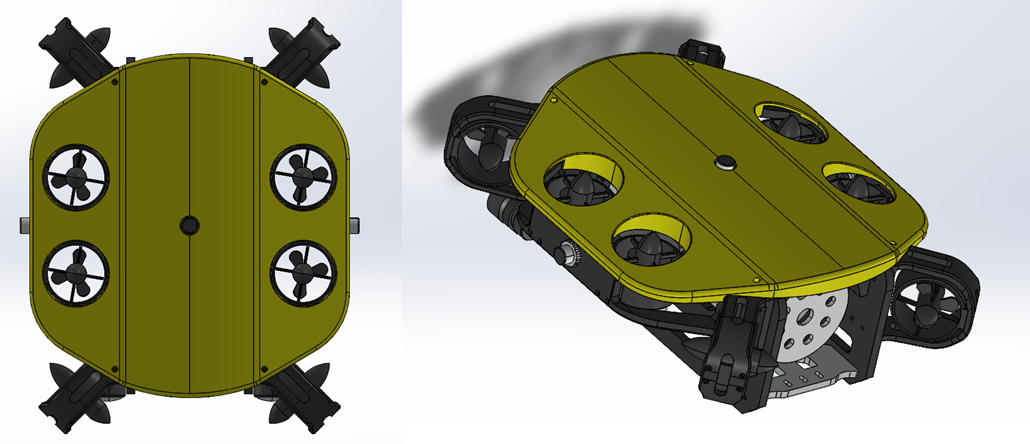
\includegraphics[width=14.5cm]{毕设图片/2-5.png}
    \caption{\label{fig:2-5}整体结构三维模型}
\end{figure}



\subsection{导流外壳设计}

导流外壳大致形状为乌龟盖形状的薄外壳,主要用于保护水下机器人内部设备免于海洋环境中的水流以及各种杂物的冲击破坏,
同时为整机提供一个水动力性能较为优秀的外形、减少运行过程中的流体阻力从而降低功耗。如\autoref{fig:2-2}所示,包括如下主要结构:
\begin{enumerate}
    \item  垂直流道:\autoref{fig:2-2}中标志1所示位置,流道沿水流方向截面为圆形,垂直推进器推动水流通过该流道为整机提供一对垂直方向推进力。
    \item  中央通孔:\autoref{fig:2-2}中标志2所示位置,上侧外壳通孔较小,主要用于方便后续改进水下机器人,例如可以用于日后水声通信装置的声头伸出从而充分与水体接触,以及用于水面定位通讯用短波天线和GPS天线伸出。
    \item  定位孔:  \autoref{fig:2-2}中标志3所示位置,用于导流壳的定位与固定。
\end{enumerate}

\begin{figure}[htbp]
    \centering
    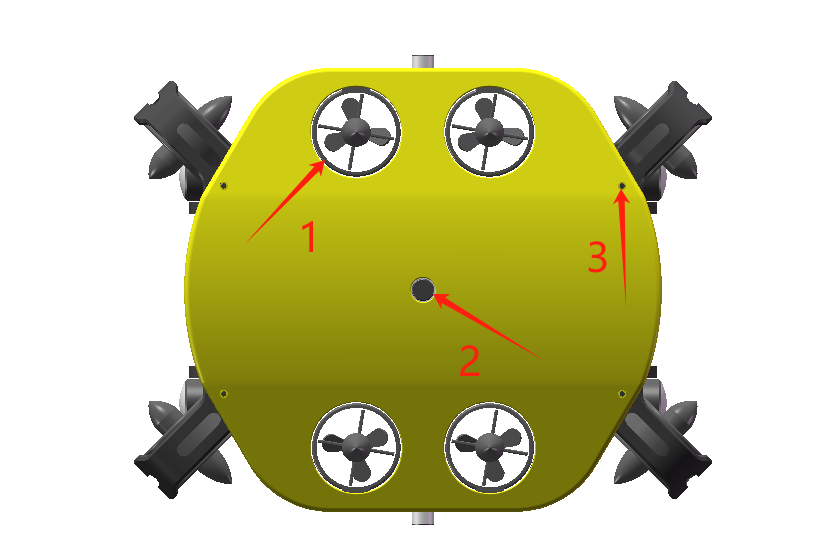
\includegraphics[width=14.5cm]{毕设图片/2-2.png}
    \caption{\label{fig:2-2}导流外壳俯视图}
\end{figure}

\subsection{骨架设计}
骨架是水下机器人内部各耐压舱体、推进器、传感器等部分的承载和固定的重要结构。在空气中,其需要有足够的强度支撑整个水下机器人结构,
在水中其需要足够的强度连接各结构,在水下机器人进行机动时,可以提供足够的力使各部件紧密结合在一起克服惯性力和流体阻力保持整体运动。

其俯视图如\autoref{fig:2-3}和整体骨架示意图如\autoref{fig:2-4}所示。为了在拥有足够强度的前提下减轻重量、方便制造、组装和运输,
采用3D打印的零部件组装而成,具体代表性零部件说明如下:
\begin{enumerate}
    \item  耐压舱固定板:\autoref{fig:2-3}中标志1所示位置,是一块3D打印的用于放置圆柱形水密控制舱的塑料件,厚度为8mm,上面的孔洞分别用于固定控制舱以及固定上部支撑架。
    \item  圆柱耐压仓固定箍:\autoref{fig:2-3}中标志2所示位置,直径为$120mm$,用于耐压舱体的固定以及内层骨架与外层骨架,内层骨架与中央板之间的连接。
    \item  防撞框架:  \autoref{fig:2-3}中标志3所示位置,主要作用是在机器人受到撞击时,更好的保护密封舱,同时负责作为垂直螺旋桨的固定支架。
    \item  垂直框架:  \autoref{fig:2-3}中标志4所示位置,用于连接防撞框架,推进器框架,同时连接耐压舱固定板,构成中间框架主体。
    \item  螺旋桨固定架: \autoref{fig:2-3}中标志5所示位置,通过螺栓紧固加紧螺旋桨。
\end{enumerate}

\begin{figure}[htbp]
    \centering
    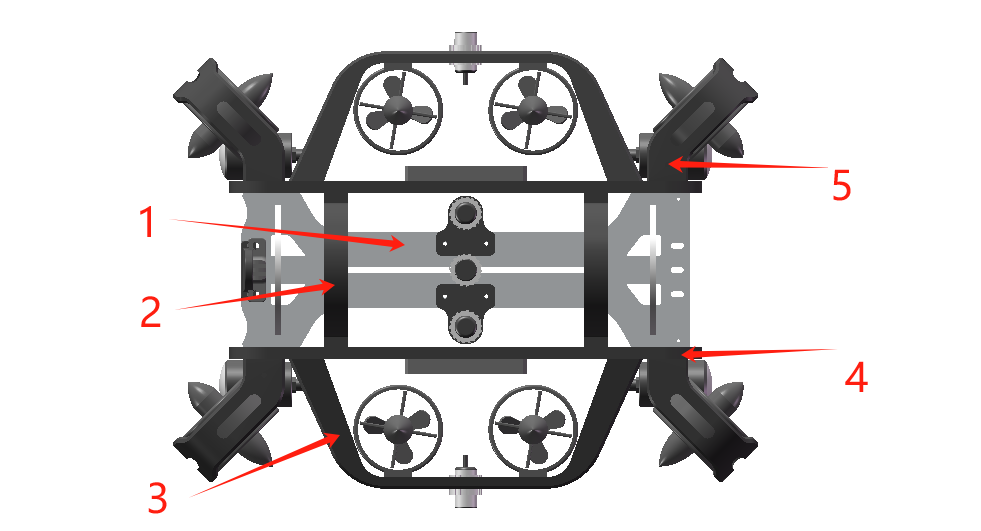
\includegraphics[width=14.5cm]{毕设图片/2-3.png}
    \caption{\label{fig:2-3}骨架俯视图}
\end{figure}

\begin{figure}[htbp]
    \centering
    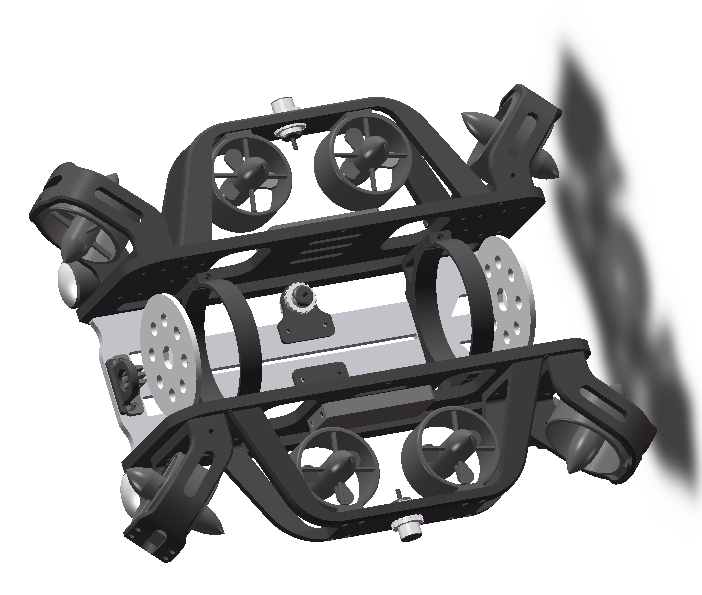
\includegraphics[width=14.5cm]{毕设图片/2-4.png}
    \caption{\label{fig:2-4}骨架结构示意图}
\end{figure}


下面写一个强度校核。

\subsection{耐压舱体设计}

耐压舱体主要为电池、控制系统硬件等设备提供保护,其要求能承受100m设计深度下的压力且保持水密特性。
由于整机的技术指标要求潜航深度100m,计算深度取技术指标的1.5倍为150m,即耐压筒的计算压力。$p_c = 1.5MPa$。
根据国家标准$GB 150.1-150.4-2011$《压力容器》对大型圆柱形耐压舱体进行设计计算。
\subsection{浮力材料}
浮力材料用于弥补机体在水中的负浮力,
根据整机设计质量与排水量估算进行选型与大致布局安装。采
用BMTI浮力材料,其相对密度为0.4。共需不超过1kg。

\subsection{推进器选型}
推进器是水下机器人在水平运动、姿态维持、定点着底工作中最重要的动力源。水下机器人中使用了四个水平的推进器和四个垂直推进器,
其中水平推进器负责提供水平运动的推进力,通过差速实现机体的零回转半径旋转等水平机动;
垂直推进器提供垂直方向推进力,用于维持直升机运动时的机体姿态,保持水平运动攻角,为小范围垂直运动提供驱动力。
\subsection{能源模块选型}
整机能源供给使用高容量锂离子电池,电池主要为推进器、控制电路以及照明装置供电。

写一个电量核算跟电池选型。


\section{硬件平台}
水下机器人硬件控制部分采用 STM32F411 微控制器控制整个系统,此处仅对系统功
能模块进行规划。供电方面,使用6串3并共18节4.2V锂电池串联构成13V直流电
源给需要的模块供电,同时将电池电压通过开关降压芯片降压到5V,再将5V电压通过线
性降压芯片降压到 3.3V 供控制系统使用,这样可以兼顾到低功耗并且减少开关电源
对模拟电路的影响。水下推进器的驱动是通过MCU输出PWM波控制电调进而控制
其和转动方向和速度,所以MCU需要输出8路PWM对8个推进器进行调速。使用
MPU9250 九轴陀螺仪及时获取姿态信息用于控制水下机器人的姿态,同时使用
MS5837 压力传感器获得机器人深度数据,用于控制机器人运动深度,MCU 需留出
IIC 接口和MPU9250以及MS5837进行通信。另外还要获取水下相关信息并上传到电
脑端,使用光电二极管获取光照强度信息,MCU感知的光照信息,输出PWM波控制
补光灯的亮度;整体结构如\autoref{fig:2-6}所示。
\begin{figure}[htbp]
    \centering
    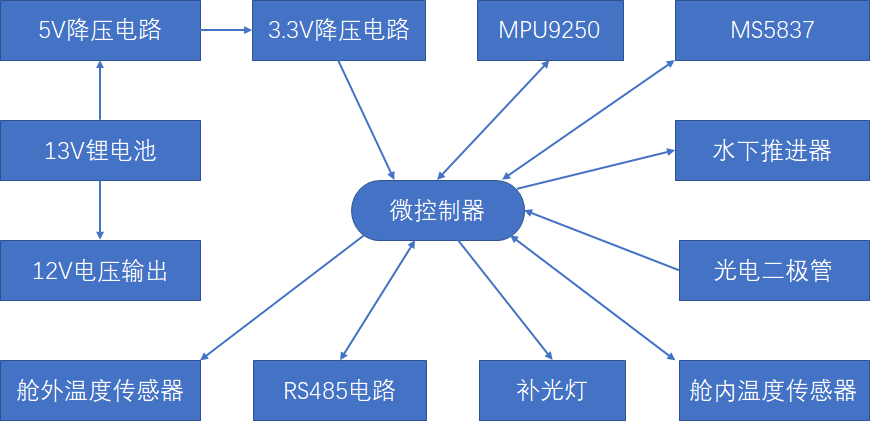
\includegraphics[width=14.5cm]{毕设图片/2-6.png}
    \caption{\label{fig:2-6}控制系统整体结构图}
\end{figure}

此硬件系统不仅需要满足水下机器人正常工作的要求,还要满足易于日后拓展的功能,
硬件软件所有功能设计应该围绕海洋生物识别的需求展开。硬件设计方
面围绕电源供电、主控、信息采集、信息传输、自动补光、异常报警等需求进行设计。
供电方面,生物识别设备和水下机器人使用同一个电源,需将电池电压转化为各个模
块所需的电压值;设计主控的最小系统保证主控芯片正常工作;使用温度传感器、湿度
传感器、MPU9250、MS5837、光敏二极管、漏水检测传感器等进行信息采集;使用
SP3485 芯片对信息传输电平进行转换;使用补光灯自动进行补光操作。硬件控制板设
计好后置于水下机器人密封舱内,硬件功能满足的前提下,对硬件功能模块的原理设
计方面没有特殊要求,只要密封舱的密封效果较好即可,但是对硬件控制电路的PCB
设计要求比较高,一方面要考虑水下机器人内的空间大小,注意舱内空间对硬件控制
电路板的尺寸限制,另一方面要保证硬件功能正常的前提下考虑 PCB 的接口位置合
理性和整体的美观性等。
\subsection{电源与电池管理板设计}
根据项目需求和功能控制电路要求,控制电路需要使用 DC5V 电源、
DC3.3V电源,水下推进器需要使用DC12V~18V电源,并且还需STM32 等芯片使用的
要有12V 的DC电压输出,本设计使用的是标13V的锂电池,需要将电池的电压进
行电压转换到各模块正常工作时的对应电压。

考虑到水下机器人使用的是锂电池供电,需要考虑到电量消耗,提高电源利用率,
减少发热,同时要考虑到主控芯片对电源纹波的要求,电源方案设计方案如下:使用开
关电源降压芯片MP2359 将13V电压降为12V和5V,然后是用线性电源AMS1117
芯片将5V降压为3.3V,经过各部分正常工作电流大小估计和芯片额定参数,电源部
分具体方案为使用 LM2576R-12 将锂电池的 13V 电压降压为 12V 电压输出、使用
MP23 59DJ-LF-Z 将锂电池的 13V 电压降为 5V 电压供电、之后使用线性降压芯片
LM1117-3.3 将 DCSV 电压转为DC3.3V。在电池组的输入输出端,有BMS电池管理模块。



\subsection{主控板设计}
\label{sec:2.3.2}
控制板主要为STM32F411CEU6及其外围传感器、驱动电路、降压电路、网络通
信端口等设计,用于获取水下机器人的水下运动姿态与深度,并通过控制算法进行自
稳定、定深度、GPS巡航等功能的实现,同时与上位机进行数据交换与通信,是最重
要的底层硬件。目前水下机器人控制系统至少需要8路PWM输出、2路ADC采集、
一个串口调试下载接口、一个SWD下载接口、一个串口收发接口(用于RS485收发收
据)、若干IO口;水下机器人目前处于样机试验研究阶段,后期会增加功能和优化功
能,必须保证主控的功能兼容性所以选用 STM32F411CEU6 作为主控芯片,
STM32F411CEU6 是 F4 系列大容量增强型产品,外设丰富,引脚更是高达 48 个,
STM32 由于其价格合理、外设丰富、功耗较低并且具有强大的软件生态支持等优点,
得到了广大开发者的认可,ST公司也因此积累了大量的用户。STM32F411CEU6工作
频率可以通过时钟源倍频到100MHz,并且内置512k字节的闪存和64K字节的SRAM,
两条APB 总线的外设上连接着多个高速 I/O 端口。最小系统电路是主控正常工作的
前提,最小系统包括供电、复位、滤波、时钟等电路,STM32有两个控制芯片启动方
式的管脚BOOT0和BOOT1,当 BOOTO接地时,正常启动;当BOOT0接3.3V,BOOT1
接地时,STM32从系统存储器启动,BOOT0, BOOT1均接3.3V时,STM32从SRAM启动。
本设计中主控制器的BOOT连接方式是BOOT0和BOOT1均接地,复位后让
STM32 正常启动。 
\begin{figure}[htbp]
    \centering
    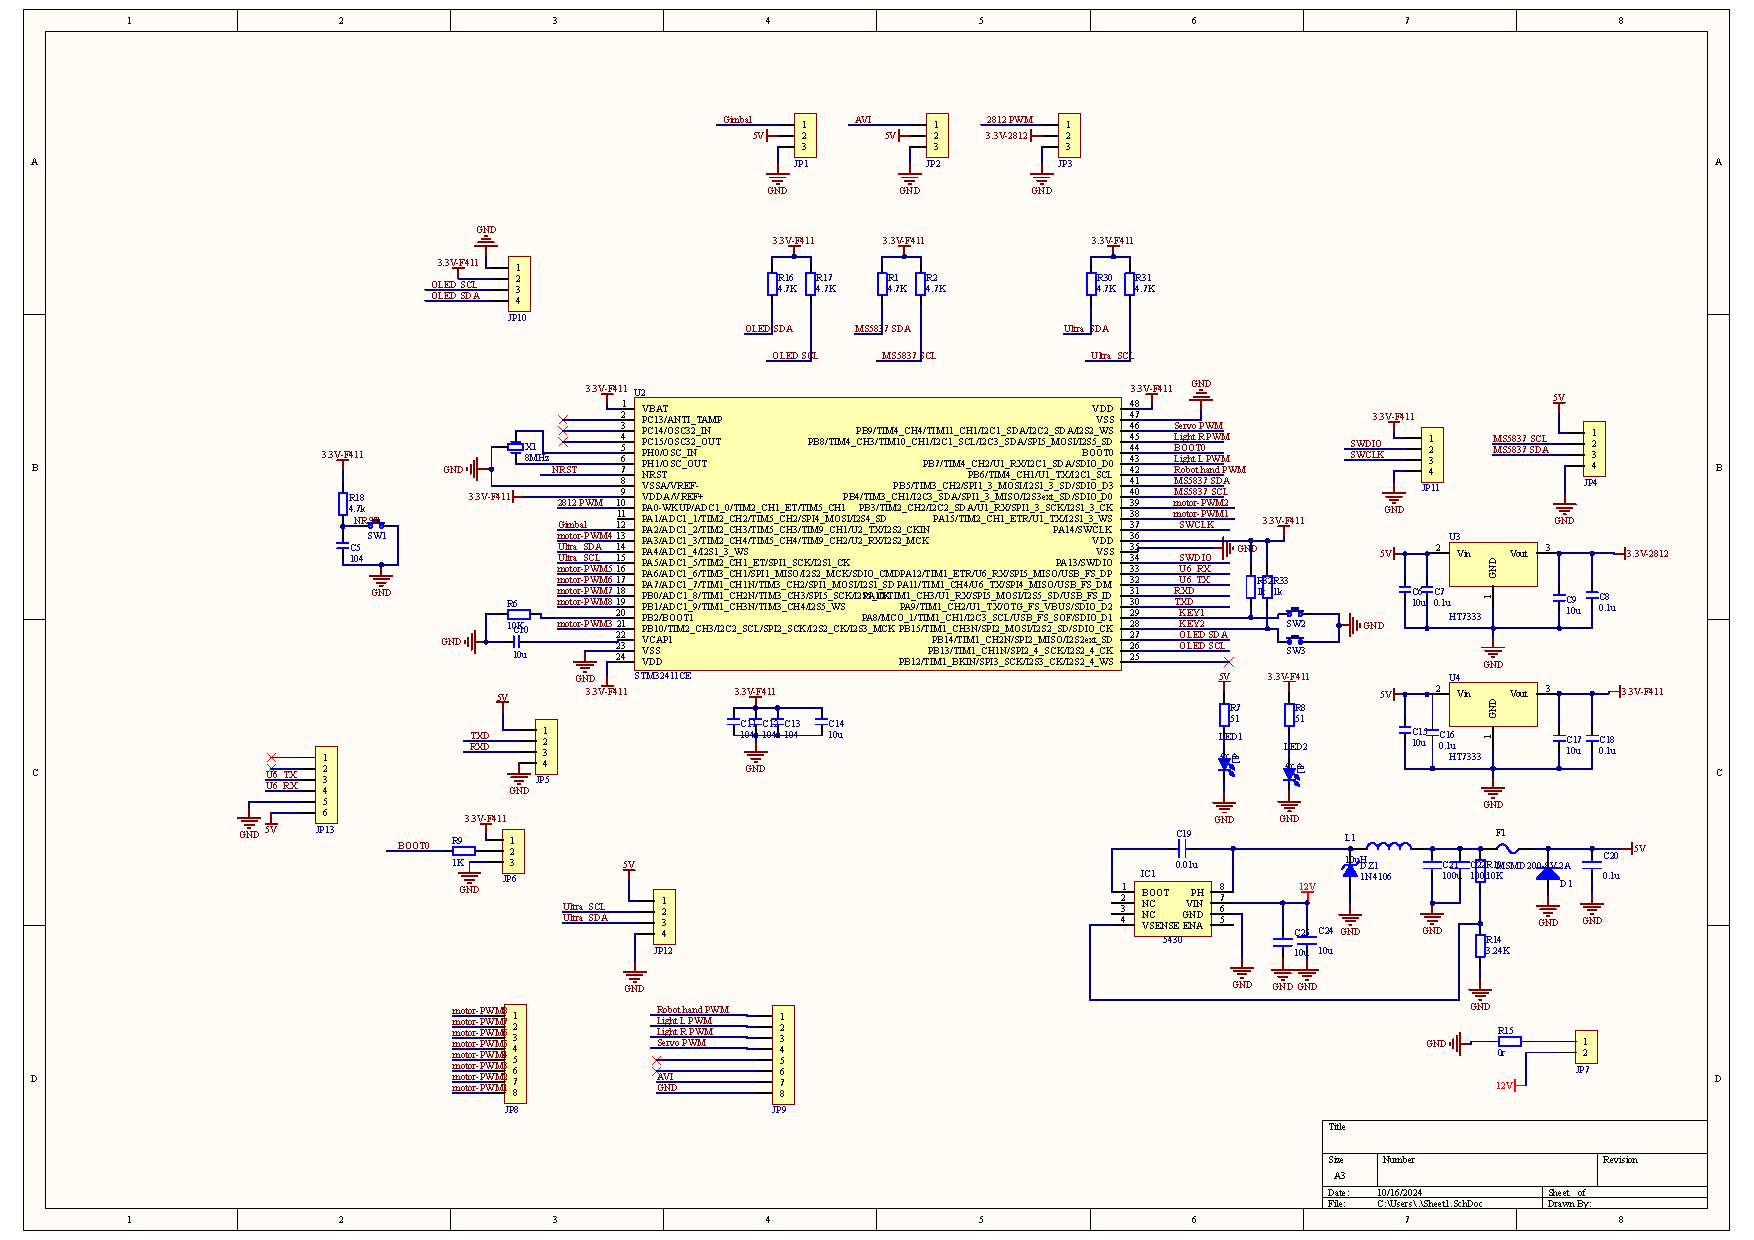
\includegraphics[width=14.5cm]{毕设图片/2-7.pdf}
    \caption{\label{fig:2-7}主控板原理图}
\end{figure}
\begin{figure}[htbp]
    \centering
    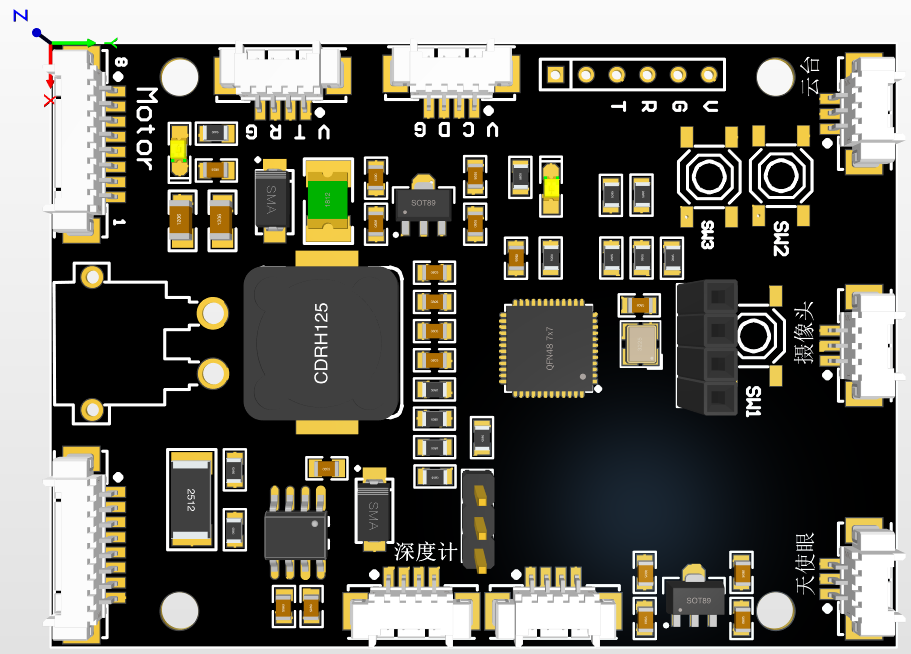
\includegraphics[width=14.5cm]{毕设图片/2-8.png}
    \caption{\label{fig:2-8}主控板PCB图}
\end{figure}

硬件复位电路的作用是为了能通过外部按键将系统从某种状态直接执进行硬复
位,按下按键后STM32的RESET引脚由高电平变为低电平触发系统复位。时钟对于
STM32 重要性就如脉搏对于人体,稳定的时钟是芯片工作的前提,本设计中通过
STM32 的 OSCIN 和 OSCOUT 引脚外接 8MHz石英晶振给系统提供时钟,系统使用
此时钟通过倍频和分频给各部分提供时钟。主控板原理图如\autoref{fig:2-7}所示,主控板PCB图如\autoref{fig:2-8}所示。

\subsection{温湿度采集模块设计}

湿度和温度是水下机器人工作时需要重点监测的信息,湿度采集是指采集水下机
器人密闭舱中的湿度信息,DTH11用于检测舱内湿度,由于在实验过程中频繁地开关
密封舱,会导致舱内湿度比空气中的湿度高,舱内电路不适宜在湿度过高的环境下工
作,长时间在湿度过高的环境下工作可能导致线路短路或者焊点加速氧化,而温度采
集包含舱外温度数据采集和舱内温度采集,舱内设备在工作时会产生较多的热量,当
舱内温度过高,则密封舱内处于相对不稳定的状态,舱内的湿度和温度过高都应该让
水下机器人停止工作,经处理状态正常后再工作。DHT11温湿度传感器是一个单总线
控制的传感器,也就是说使用一个IO口就可以控制DTH11,可通过该IO口将温度
和湿度信息读出。为保证数据的准确性,DHT11传输的数据都有1 Byte 数据用于校
验。它的温度测量范围为。0$\backsim $50摄氏度,误差达2摄氏度,无法测量零度以下温度,
湿度测量范围为20\%$\backsim$90\%,湿度测量精度为正负5\%,很明显,DTH11温度测量精度不
如价格更便宜的DS18B20,所以舱内外温度测量均使用是DS18B20,DHT11仅用于
测量湿度。 

DHT 11 的传输时序对于编写DHT11驱动程序是至关重要的,主机将总线拉低
并保持18ms以上为开始信号,再将总线拉高20$\backsim$40us,然后等待DHT11的响应,在
传输数据过程中DTH11再将总线拉低12$\backsim14$us 之后将总线拉高26$\backsim28$us 表示传输数
字“0",如果拉低12$\backsim$14us 后拉高116$\backsim$118us 则表示传输数字“1"。DHT11 输出的数据
包一共包含40个bit共5Byte,传输时高位先出,5Byte数据的意义分别为:byte4,byte3
为湿度数据,byte2, byte1 为温度数据、byte0 为用于校验的校验和,byte2,byte 1,
byte3,byte4 相加的和byte0 相等,则代表数据读取正常。DHT11 电路设计与布局如\autoref{fig:2-9}所示。
\begin{figure}[htbp]
    \centering
    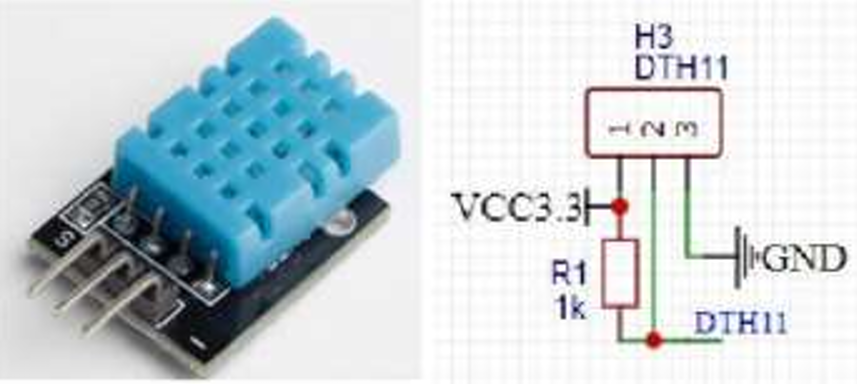
\includegraphics[width=14.5cm]{毕设图片/2-9.png}
    \caption{\label{fig:2-9}DHT11 电路设计与布局}
\end{figure}

DS18B20 相对于常用的热敏电阻体积更小、适用电压更宽、不需要复杂的外围硬
件电路,和DTH11一样只需要一个微控制器的IO口便可以读出温度值,而使用传统
的热敏电阻测量温度需要更多的外围电路,无形中增加了测量的器件成本和设计成本,
也不利于节约 PCB 板面面积,可能还要将模拟的电流或者电压处理后变成主控能识
别的数字量。DS18B20的测量温度范围广精度高,多种封装方式可满足多种场景需求,
本设计舱内温度传感器使用直插式封装,舱外温度传感器使用的是 DS18B20 是可以
水下测量的封装。其读写方式和DTH11类似,在此不做赘述。舱内舱外温度采样电路如\autoref{fig:2-10}所示。
\begin{figure}[htbp]
    \centering
    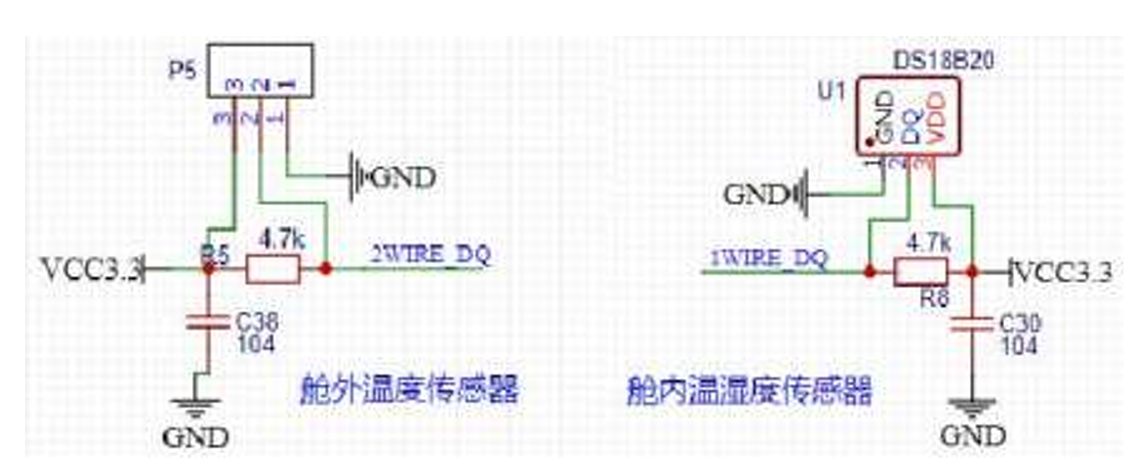
\includegraphics[width=14.5cm]{毕设图片/2-10.png}
    \caption{\label{fig:2-10}DHT11 舱内舱外温度采样电路}
\end{figure}

\subsection{光照信息采集部分和补光灯部分}

当水下光照条件不好的情况下,水下机器人搭载的图像处理设备获取的照片和视
频成像质量会下降,直接影响图像识别的效率和效果。当水下光照度下降一定值时,
获取的图像将无法被识别,所以需要光照传感器获取水下光照强度并将信息传输到主
控板,主控板接收到光照信息后控制水下补光灯的工作,以满足摄像机成像所需光照
要求。
\begin{table}[H]
    \fangsong
    \caption{\label{tab:2-1}水下照明补光LED灯参数}
    \small %此处写字体大小控制命令
    \centering%把表居中
    \renewcommand{\arraystretch}{1.5}
    \setlength{\tabcolsep}{3mm}{
    \begin{tabular}{ccccc}
    \toprule%第一道横线位姿 
    属性 &特性\\
    \midrule%第二道横线 
    防水深度  &  小于或等于200米 \\
    外壳材质 &	铝合金硬质氧化 \\
    亮度 &	    1500流明\\
    色温 &	6500K \\
    供电 &	 12 $\backsim$ 36 伏特\\
    控制接口&	 PWM \\
    重量& 空气中165克,水下125克\\
    线长&1米\\
    功率&15瓦\\
    \bottomrule%第三道横线
    \end{tabular}}
\end{table}

补光灯使用PWM控制的铝合金硬质深水防水高亮度LED灯,该补光灯专为水
下环境设计,额定功率15W,色温6500K,亮度1500流明,非常适合水下成像补光,
STM32F411CEU6 通过PF8引脚采集光照接收部分的电压值,补光灯的亮度调节可根
据采集到的光照量化值,在对应引脚上输出合适的PWM波形来实现调节补光灯的光
照强度。大功率LED驱动XL6006照明电路如\autoref{fig:2-11}所示。
\begin{figure}[htbp]
    \centering
    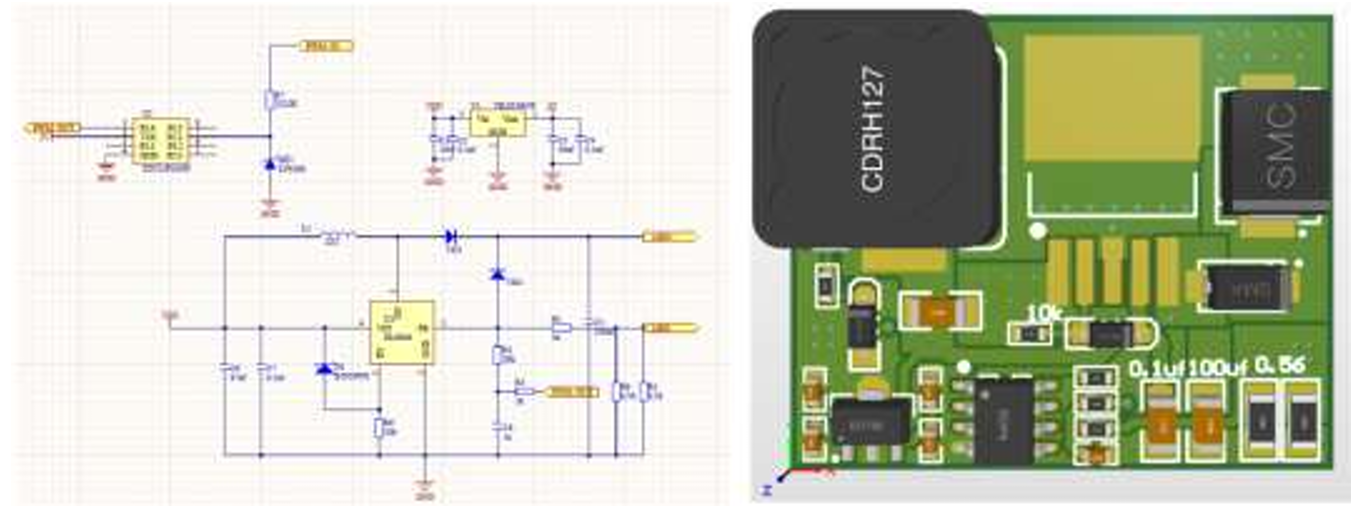
\includegraphics[width=14.5cm]{毕设图片/2-11.png}
    \caption{\label{fig:2-11}大功率LED驱动XL6006照明电路}
\end{figure}
水下照明补光LED灯参数如\autoref{tab:2-1}所示,实物图如\autoref{fig:2-12}所示。

\begin{figure}[htbp]
    \centering
    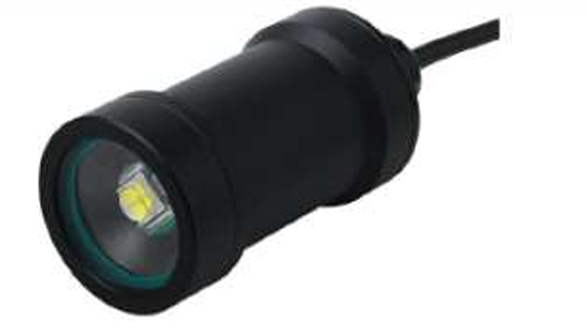
\includegraphics[width=14.5cm]{毕设图片/2-12.png}
    \caption{\label{fig:2-12}水下照明补光LED灯实物图}
\end{figure}
\subsection{姿态控制传感器}
水下机器人在水下运动时通过控制板对水下推进器的控制,要准确地感知水下机
器人的运动姿态,并根据其姿态信息及时做出反应,必须使用姿态感知传感器实时获
取水下机器人姿态,姿态感知传感器使用MPU9250九轴传感器。和其他解决方案相
比,MPU9250更小的功耗、更小的封装、更准确的传感、更少的组件、更好控制的接
口以及更便宜的价格使得MPU9250得到越来越多的工程师的青睐。

MPU9250 能通过IIC接口以数字的形式输出旋转矩阵、四元数、欧拉角格式的融
合验算数据,自带1024字节FIFO,降低了系统处理数据的功耗,数据读取更快更便
捷,超小尺寸QFN封装,简洁的外围硬件电路,大大节省了硬件板面面积。我们能清
晰看到 MPU9250 几个重要的引脚,MCU 通过可以 SCL 和 SDA 两个引脚来控制
MPU9250。从框图中可看到,实际上MPU9250 是通过7路ADC采集的方式,将重力加速度、
姿态角、温度的信息转换为电路能识别的电信号,通过数据调节后将数据
存到相应的寄存器中,MCU对MPU9250内部数据寄存器的读操作可读出姿态数据,
对MPU9250的配置寄存器读写可以设置工作状态和实时获取运动器姿态信息。其内部框图如\autoref{fig:2-13}所示。
\begin{figure}[htbp]
    \centering
    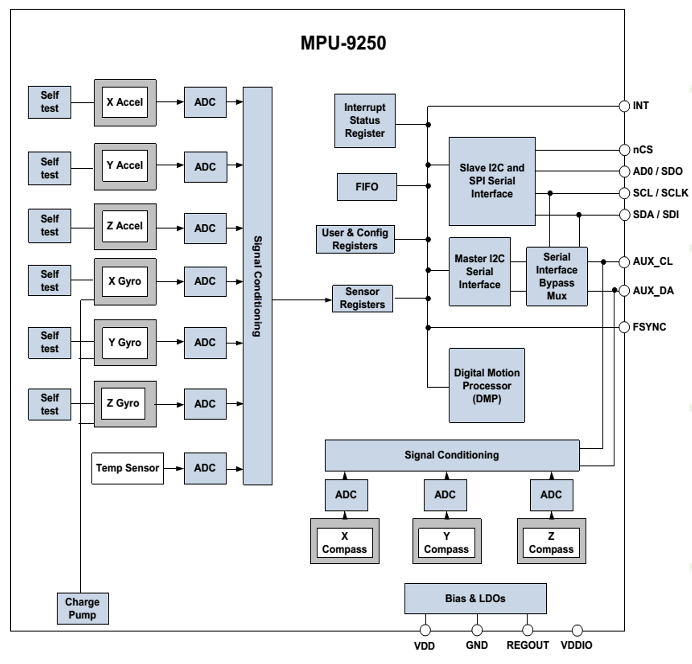
\includegraphics[width=14.5cm]{毕设图片/2-13.png}
    \caption{\label{fig:2-13} MPU9250内部框图}
\end{figure}

\subsection{通信板设计}

采用2.4G频率发射接收模块和5.8G频率发射接收模块,分别发射接收控制信号
和图像,采用无刷电机驱动板和stm32最小系统板。RS-485总线标准规定利用两根传
输线间的电压差的方式来区分传输信息的逻辑,外部干扰对两根差分线中传输数据的
影响可以近似认为是相同,在接受端识别逻辑的方式是两个传输线上的电压做减法,
因此传输逻辑基本不受影响,这种差分传输形式的能有效抑制了大部分类型的干扰,
被广泛用于工业控制自动化等复杂场景,其特点如下:  
\begin{itemize}
    \item 采用差分传输方式,传输抗干扰能力强。
    \item 数据最高传输速率可以达到10Mbps。 
    \item 理论最多可连接一百多个设备,便于设备组网通信。
    \item 理论最大传输距离大约3000米。
\end{itemize}
RS485电路原理图与PCB图如\autoref{fig:2-14}所示。
\begin{figure}[htbp]
    \centering
    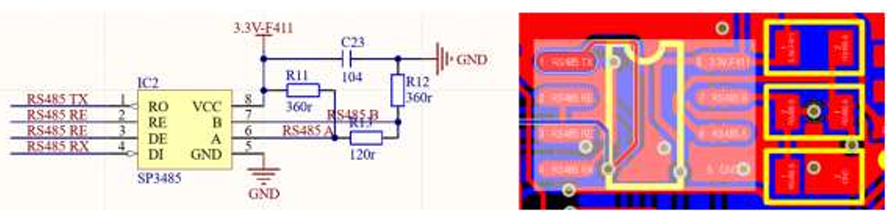
\includegraphics[width=14.5cm]{毕设图片/2-14.png}
    \caption{\label{fig:2-14} RS485电路原理图与PCB图}
\end{figure}
\subsection{电调设计}
先放着决定要不要写,看看有没有原图。
\section{底层软件设计}
底层嵌入式软件的设计主要是基于\ref{sec:2.3.2}节中的底层主控板设计来实现的。
主要包括传感器设备例如九轴姿态传感器的初始化以及通信协议,中断控制逻辑、
基本的定时器、PWM控制水下推进器等内容。软件的编写主要使用的是C语言,开发软件使用的是Keil uVision 5。

Keil uVision 5 是一款由 ARM Keil 开发的专业集成开发环境(IDE),
主要用于基于 ARM Cortex-M 微控制器的程序开发。它提供了一个完整的 IDE,支持从编写源代码到编译、链接以及最终调试整个开发流程。
编辑器具备语法高亮、代码折叠、自动补全等功能,提高编码效率。编译器内置了高效的 ARM 编译器,能够将 C/C++ 代码编译成优化后的机器码。
调试器支持硬件断点、查看变量值、单步执行、修改内存等调试功能。可以与目标硬件上的调试硬件(如 J-Link 或 SWD)通信,进行非侵入式的实时调试。
在项目管理方面,它支持创建和管理多个工程文件,每个工程文件可以包含多个源文件和对象文件同时提供了多种视图,
如 Project Explorer、Symbol Browser、Call Graph 等,便于开发者浏览项目结构、函数调用关系等。此外,它可以与第三方工具和服务集成,
扩展开发环境的功能,支持多种 ARM Cortex-M 系列微控制器,并且与之前的 Keil MDK 版本兼容,允许用户平滑过渡到新版本。总的来说,
它集成了项目管理、代码编辑、编译、调试等多种功能于一体,使得开发者可以更加高效地进行嵌入式系统的开发工作,可以更快速地开发稳定可靠的嵌入式软件。

软件采用FreeRTOS(Free Real-Time Operating System)操作系统。
FreeRTOS是一款广受赞誉的实时操作系统(RTOS),专为嵌入式系统设计。
自2003年由Richard Barry首次发布以来,
FreeRTOS 已经成为嵌入式开发者的首选操作系统之一。
2018年,FreeRTOS 被亚马逊收购,并更名为 AWS FreeRTOS,进一步增强了其在物联网(IoT)领域的应用能力。其特点如下:
\begin{itemize}
    \item FreeRTOS 的一大特色在于它是完全免费且开源的,遵循 MIT 许可证,
    任何人都可以自由下载、使用、修改和分发 FreeRTOS 的源代码,无需支付任何费用。
    这对于预算有限的个人开发者来说极具吸引力,因为它降低了嵌入式项目的初始成本。
    \item FreeRTOS 设计的极其轻巧,其核心代码量极小,通常不超过几千行。
    这样的设计使得 FreeRTOS 能够在资源极其有限的微控制器上运行,例如仅有几KB RAM 和几十KB ROM 的设备。
    这一点对于需要实时响应并且硬件资源受限的嵌入式应用至关重要。 
    \item FreeRTOS 采用了模块化的设计思路,允许开发者根据实际需求选择需要的功能模块。
    用户可以根据自己的应用环境来裁剪 FreeRTOS,移除不必要的组件,从而进一步减少内存占用。
    这种灵活性使得 FreeRTOS 成为广泛应用于不同领域的理想选择。
    \item 作为一款实时操作系统,FreeRTOS 提供了确定性的响应时间。
    它采用了优先级调度算法来管理任务(thread),确保高优先级的任务能够在低优先级任务之前获得执行的机会。
    这种机制使得 FreeRTOS 能够快速响应外部事件,非常适合那些需要实时处理输入输出数据的应用场合。
    \item 在 FreeRTOS 中,任务是最基本的执行单元。
    开发者可以创建多个任务,并为每个任务赋予不同的优先级。
    此外,FreeRTOS 还提供了一系列任务间通信和同步机制,如信号量(semaphore)、消息队列(message queue)、互斥锁(mutex)等。
    这些机制帮助开发者实现任务间的协同工作,确保数据的一致性和完整性。
    \item 尽管 FreeRTOS 本身并不提供复杂的内存管理功能,
    但它允许开发者使用自定义的内存管理方案。
    FreeRTOS 支持动态内存分配,但也鼓励开发者使用静态内存分配来避免内存碎片问题,
    提高系统的稳定性和响应速度。
    \item FreeRTOS 对中断处理给予了特别的关注,支持在中断服务程序(ISR)中执行快速响应操作。
    中断服务程序可以使用信号量等手段与普通任务进行通信,从而实现在中断发生时的高效处理。
    \item FreeRTOS 可以运行在多种不同的微控制器架构上,包括但不限于 ARM Cortex-M、RISC-V、MIPS 等。
    这种广泛的硬件兼容性使得 FreeRTOS 成为跨平台开发的理想选择,开发者可以在不同的硬件平台上复用相同的软件代码。
    \item FreeRTOS 还拥有一个庞大而活跃的开发者社区,成员们积极贡献代码、分享经验,并提供技术支持。
    此外,FreeRTOS 官方还提供了详细的文档和教程,帮助新手快速上手。
    对于那些寻求商业支持的企业用户,市面上也有不少第三方服务商提供基于 FreeRTOS 的技术支持和服务。
\end{itemize}


基于FreeRTOS的诸多优点,FreeRTOS 已经广泛应用于多个领域,包括但不限于工业自动化、智能家居、医疗设备、汽车电子、消费电子产品等领域。
随着物联网技术的快速发展,FreeRTOS 的应用范围还将进一步扩大。Amazon 收购 FreeRTOS 后,
增加了对物联网的支持,使其能够更好地与其他云服务集成。
未来,FreeRTOS 有望在连接嵌入式设备与云端服务方面发挥更大作用,推动嵌入式系统向智能化方向发展。

\subsection{传感器驱动与数据采集程序 }
深度传感器的型号是MS5837-30BA,采用IIC通信,内部有一个112位的PROM,用于补偿工艺和温度变化所必需的六个系数
经过计算存就储存在这里。主控板通过输入串行时钟(SCL)和串行数据(SDA)对数据进行时间记录。
该传感器在同一引脚 SDA 上响应,该引脚 SDA 对于 IIC 总线接口是双向的,因此该类型接口仅使用两根信号线,不需要片选。
通过IIC通信,主控板对其进行复位等操作。每条 IIC 通信消息以启动条件开始,以停止条件结束。MS5837-30BA 地址是1110110x,
其中x代表0或1,当x为0时,代表的时写指令,
当x为1时,代表的是读指令,即写指令为0xEC,读指令为0xED。

在我们使用深度传感器时,我们发送写指令后,还需要对其发送对应的命令,这些命令以十六进制值表示,
这样才能对深度传感器进行我们需要的操作,MS5837只有五个基本命令,如\autoref{tab:2-2}所示。
根据发送的十六进值的不同,MS5837-30BA会执行不同的操作。
\begin{table}[H]
    \fangsong
    \caption{\label{tab:2-2}MS5837 十六进制值与对应的功能}
    \small %此处写字体大小控制命令
    \centering%把表居中
    \renewcommand{\arraystretch}{1.5}
    \setlength{\tabcolsep}{3mm}{
    \begin{tabular}{ccccc}
    \toprule%第一道横线位姿 
    十六进值 &对应功能\\
    \midrule%第二道横线 
    0X1E   &  复位  \\
    0XA2-0XAC  & 读取出厂校准值C1-C6  \\
    0X48  &	    数据D1转换(压力值数据) \\
    0X58  &	    数据D2转换(温度值数据)\\
    0X00  &	    读ADC转换结果(24 位温度值与压力值)\\
    \bottomrule%第三道横线
    \end{tabular}}
\end{table}
具体使用过程,就是打开电源开关,深度传感器进行初始化,接着读取校准参数,保存下初始的
压力值与温度用于后续深度计算。
在读取深度的过程中,首先需要进行数据D1与D2
转化,随后发送读ADC转换结果指令,得到温度与压力值信息,根据官方提供的二阶
补偿公式计算得到当前时刻水下机器人的深度信息,其代码流程图如\autoref{fig:2-15}所示。
\begin{figure}[htbp]
    \centering
    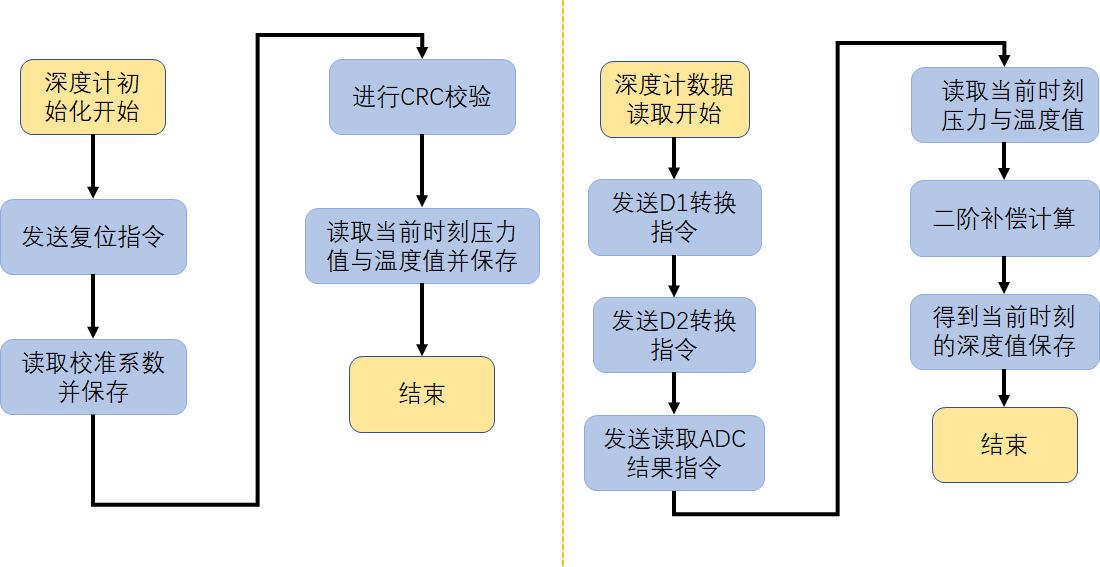
\includegraphics[width=14.5cm]{毕设图片/2-15.png}
    \caption{\label{fig:2-15} 深度计初始化及数据读取流程图}
\end{figure}

姿态传感器使用的是MPU-9250,采用IIC通信,有SDA和SCL两根线分别传输数据和时钟信号。
MPU-9250在本项目中是作为从机进行通信,SDA和SCL上拉电阻到VDD,
通过地址进行匹配。MPU-9250作为从机通信时,它的地址为7位110100X(B),这个地址的LSB位由AD0引脚的电平确定,
这样就可以在一个系统里面同时连接两个MPU-9250,AD0为高电平时,x为1,AD0为低电平时,x为0。在进行数据传输时,IIC每帧数据包含8位
数据位和一位(ACK)数据接收方应答位。从机负责应答位ACK的拉低,当从机正确接收到数据时,从机会拉低SDA总线。

在开始信号发出后,主机开始发出7个地址位和1个读写位。读写位决定了
主从机的读写状态。然后主机释放SDA线,等待从机的ACK应答信号。每次
数据传输后必须跟一位读写位。从机应答即是拉低SDA到SCL高电平周期结
束。当主机发出停止命令时,传输就会结束。然后主机重新发送开始信号继
续和其他的IIC设备通信。当SDA出现上升沿并且SCL是高电平的时候,就
表示停止信号。在通信时所有SDA信号的变化都是在SCL低电平的时候。

写MPU250 的寄存器的方法:主机发送开始信号和从机的 7 个地址位再加上1
位的写入位。当在第9个时钟信号的时候,芯片产生应答。这时,主机输出寄
存器地址,然后从机再次产生 ACK 应答,传输过程可以随时由停止信号停止。
ACK 响应后,数据可以继续输入,除非没有产生停止位。芯片内部自带的递增
寄存器可以自动将数据写入相应寄存。以下列出单字节和双字节的传输顺序。

读MPU9250 的寄存器的方法:主机发送开始信号和从机的7个地址位再加上读
位。此时,寄存器地址变成可读模式。此时会收到MPU9250的返回信号ACK,
然后主机再次发送开始信号和地址,9250此时会发回应答信号ACK和数据。当
主机发送NACK或停止位后通讯停止。NACK信号就是第9个时钟脉冲SDA保持
高电平。下图显示了单字节和双字节的读取时序。

在具体的使用过程中,IIC 通信的实现是通过软件模拟的方式进行的,
即所谓的“软件IIC”。这种方式通过控制 GPIO 引脚的状态来模拟 IIC 
通信所需的信号,包括起始、停止、数据传输和应答等。所以需要首先进行IIC的初始化,例如使能GPIO时钟、GPIO口初始化等。
然后通过操作MPU-9250的寄存器实现复位MPU-9250、唤醒MPU-9250、设置MPU9250陀螺仪传感器满量程范围、设置MPU9250加速度传感器满量程范围、设置采样率50Hz、
关闭所有中断等功能,完成MPU-9250的初始化。接着就可以根据协议读取返回的数据内容,进而对数据内容进
行处理并且保存。 

\subsection{执行器驱动 }
水下机器人的执行器分别为水下推进器、水下照明灯、舵机。在对水下机器人操作的过程中,首先先进行PWM的初始化,接着设置PWM的频率,最后设置占空比。
根据占空比来控制水下推进器的旋转。其中1500是停止。大于等于1000小于1500是反转,大于1500小于等于2000是正转。
根据控制输出的数据,确定对应的推进器的PWM信号的脉冲宽度,
进而控制每个推进器的旋转方向跟旋转速度。

\subsection{底层主控框架与流程}
% \section{引言}

% \section{标定算法框架}

% 本文提出了一种适用于水下双目相机标定的坐标约束算法,目标是求解水下双目相机折射参数,水下双目相机通常需要封装在一个耐压舱体中,相机前端通常使用玻璃或者亚克力板等透明耐压介质。因此,需要求解舱体玻璃表面法线的在相机坐标系下的方向向量、玻璃表面内侧到相机光芯的距离以及玻璃的厚度,如\autoref{fig:2-2}(a)所示。具体来说,相机封装之前使用张氏标定 法获取立体相机的内参矩阵和外部参数矩阵,然后封装好水下相机,在水下从各种角度拍摄棋盘,并提取左右相机图像上的棋盘角点的像素坐标,通过折射模型计算水中空间点的坐标。如\autoref{fig:2-2}(c)所示,当已经获得相机坐标系下的所有棋盘格三维点位置时,将这些点建立一个独立的坐标系,并拟合标准棋盘格坐标系,构建误差函数,最后使用非线性优化的方法找到最优解。

% \section{水下双目成像建模}

% 针对水下双目相机,本节推导出水下双目成像模型,使用\autoref{tab:1}中的符号去描述这一过程。
% %经典三线表
% \begin{table}[H]
%     \fangsong
%     \caption{\label{tab:1}折射描述符号}
%     \small %此处写字体大小控制命令
%     \centering%把表居中
%     \renewcommand{\arraystretch}{1.5}
%     \setlength{\tabcolsep}{8mm}{
%     \begin{tabular}{m{2cm}m{9cm}}
%     \toprule%第一道横线
%     符号 & 解释说明    \\ 
%     \midrule%第二道横线 
%     ${{\bf{K}}_l,{\bf{K}}_r}$  & 左相机和右相机的内参矩阵              \\
%     ${d_{1l},d_{1r}}$  & 分别从左相机和右相机的光芯到玻璃内侧表面的垂直距离                     \\
%     ${d_2}$  & 耐压玻璃板的厚度                    \\
%     ${{\bf{v}}_l},{{\bf{v'}}_l},{{\bf{v''}}_l}$  & 左相机像素点对应的光线:从相机光芯到玻璃板内侧,玻璃板内部,玻璃板外侧到水中             \\
%     ${{\bf{v}}_r},{{\bf{v'}}_{\rm{r}}},{{\bf{v''}}_r}$  & 右相机像素点对应的光线               \\
%     ${\theta _l},{\theta '_l},{\theta ''_l}$  & 左相机像素点对应的光线与玻璃板法线的夹角:舱内空气中的光线,玻璃板中的光线,水中的光线            \\
%     ${\theta _r},{\theta '_r},{\theta ''_r}$  & 右相机像素点对应的光线与玻璃板法线的夹角    \\
%     ${{\bf{P}}_{la}},{{\bf{P}}_{lb}}$  & 和玻璃板内侧的交点和玻璃板外侧的交点 \\
%     ${{\bf{P}}_{ra}},{{\bf{P}}_{rb}}$  & 和玻璃板内侧的交点和玻璃板外侧的交点   \\
%     ${{\bf{n}}_l},{{\bf{n}}_r}$ & 玻璃板的法线在左相机和右相机坐标系下的坐标  \\
%     ${\rho _0},{\rho _1},{\rho _2}$ & 空气,玻璃和水的折射参数 \\
%     ${\bf{R}}$ & 右相机坐标系变换到左相机坐标系的旋转矩阵          \\
%     ${\bf{t}}$ & 右相机坐标系变换到左相机坐标系的平移矩阵         \\
%     ${{\bf{P}}_{i,j}}$ & 标定板的第i行第j列                   \\
%     ${{\bf{P'}}_{i,j}}$ & 通过双目相机计算的标定板的第i行第j列                   \\
%     \bottomrule%第三道横线
%     \end{tabular}}
%     \end{table}

% 如\autoref{fig:2-2}(a)所示,本文以右相机为例描述水下双目相机成像过程。相机像素坐标与归一化坐标满足以下关系:
% % \begin{equation}
% %     \label{equ:2-1}
% %     \mathbf{v}_r=\left[\begin{array}{l}u_c \\ v_c \\ 1\end{array}\right]=\mathbf{K}\left[\begin{array}{l}x \\ y \\ 1\end{array}\right], \mathbf{K}=\left[\begin{array}{ccc}f_x & 0 & c_x \\ 0 & f_y & c_y \\ 0 & 0 & 1\end{array}\right]
% % \end{equation}
% 其中,归一化坐标即为像素点对应的舱内空气的光线向量${{\bf{v}}_l}$,内参矩阵${\bf{K}}$由张氏标定法计算得到,${f_x}$和${f_y}$为$x$和$y$方向上的焦距,${c_x}$和${c_y}$为$x$和$y$方向上的主点偏移量。当已知右相机光芯到玻璃面的距离${d_{1r}}$时,在相机坐标系下的${{\bf{v}}_r}$和玻璃板内侧的交点${\bf{P_{ra}}}$为:
% \begin{equation}
%     \label{equ:2-2}
%     {\bf{P_{ra}}} = {{\bf{v}}_r} \cdot \frac{{{d_{1r}}}}{{{{\bf{v}}_r} \cdot {{\bf{n}}_r}}}
% \end{equation}

% 下面根据折射Snell定律求解折射后对应的玻璃的光线向量${\bf{v'}}$。光线跨介质传输时满足以下定律:
% \begin{equation}
%     \label{equ:2-3}
%     \sin {\theta '_r}{\rho '_r} = \sin {\theta _r}{\rho _r}
% \end{equation}
% 其中,${\theta _r}$为空气中光线与交界面法线的夹角,${\rho _0}$为空气的折射系数,${\theta _r}^\prime $为出射光线与交界面法线的夹角,${\rho _1}$为玻璃介质的折射系数。Snell定律用向量表示为:
% \begin{equation}
%     \label{equ:2-4}
%     {{\bf{v'}}_{\rm{r}}} = a{{\bf{v}}_r} + b{{\bf{n}}_r}
% \end{equation}
% 其中
% \begin{equation}
%     \label{equ:2-5}
%     a = {{{\rho _0}} \mathord{\left/
%  {\vphantom {{{\rho _0}} {{\rho _1}}}} \right.
%  \kern-\nulldelimiterspace} {{\rho _1}}}
% \end{equation}
% \begin{equation}
%     \label{equ:2-6}
%     b = \frac{{ - {\rho _0}{\bf{v}}_r^T{{\bf{n}}_r} - \sqrt {\rho _0^2{{\left( {{\bf{v}}_r^T{{\bf{n}}_r}} \right)}^2} - \left( {\rho _0^2 - \rho _1^2} \right){\bf{v}}_r^T{{\bf{v}}_r}} }}{{{\rho _1}}}
% \end{equation}

% 当已知玻璃板中的交点和向量后,再次应用式 \eqref{equ:2-4}就能确定水中光线的具体坐标,从而求出${{\bf{P}}_{rb}},{{\bf{v''}}_r}$。已知右相机的折射参数后,可以根据右相机和左相机的坐标转换关系求出左相机坐标系下的折射参数。
% 其中,左相机坐标系下的法线为:
% \begin{equation}
%     \label{equ:2-7}
%     {{\bf{n}}_l} = {\bf{R}}{{\bf{n}}_r}
% \end{equation}
% 左相机光芯与玻璃面的距离为:
% \begin{equation}
%     \label{equ:2-8}
%     {d_{1l}} = {d_{1r}} + {\bf{t}} \cdot {{\bf{n}}_r}
% \end{equation}
% 同样可以求出左相机像素点对应的在水中的光线向量${{\bf{v''}}_l}$和交点${{\bf{P}}_{lb}}$。

% 下面计算两相机对应的水中的光线的交点。首先,将右相机坐标系下的向量和交点变换到左相机坐标系下。左相机坐标系下的光线向量为:
% \begin{equation}
%     \label{equ:2-9}
%     {{\bf{v''}}_{lr}} = {\bf{R}}{{\bf{v''}}_r}
% \end{equation}
% 左相机下的交点坐标为:
% \begin{equation}
%     \label{equ:2-10}
%     {{\bf{P}}_{lrb}} = {\bf{R}}{{\bf{P}}_{rb}} + {\bf{t}}
% \end{equation}
% 考虑误差存在的情况,两条光线不一定会相交,取相交并垂直于两条光线的线段的中点作为其交点,记做$\bf{m}$,有
% \begin{equation}
%     \label{equ:2-11}
%     {\bf{m}} \cdot {{\bf{v''}}_{lr}} = 0
% \end{equation}
% \begin{equation}
%     \label{equ:2-12}
%     {\bf{m}} \cdot {{\bf{v''}}_{l}} = 0
% \end{equation}
% 向量$\bf{m}$是通过该垂直线段确立的,垂直线段的起点记为$\bf{M1}$,位于左相机对应的光线上;终点记为$\bf{M2}$,位于右相机对应的光线上。记${{\bf{P}}_{lrb}}{{\bf{P}}_{lb}}$的连线为${\bf{I}}$,则有以下公式:
% \begin{equation}
%     \label{equ:2-13}
%     {{\bf{M}}_1} = {{\bf{P}}_{lb}} + {{\bf{v''}}_l}\frac{{ - \left( {{{{\bf{v''}}}_l} \cdot {{{\bf{v''}}}_{lr}}} \right)\left( {{{{\bf{v''}}}_{lr}} \cdot {\bf{I}}} \right) + \left( {{{{\bf{v''}}}_l} \cdot {\bf{I}}} \right)\left( {{{{\bf{v''}}}_{lr}} \cdot {{{\bf{v''}}}_{lr}}} \right)}}{{\left( {{{{\bf{v''}}}_l} \cdot {{{\bf{v''}}}_l}} \right)\left( {{{{\bf{v''}}}_{lr}} \cdot {{{\bf{v''}}}_{lr}}} \right) - \left( {{{{\bf{v''}}}_l} \cdot {{{\bf{v''}}}_{lr}}} \right)\left( {{{{\bf{v''}}}_l} \cdot {{{\bf{v''}}}_{lr}}} \right)}}
% \end{equation}
% \begin{equation}
%     \label{equ:2-14}
%     {{\bf{M}}_2} = {{\bf{P}}_{lrb}} + {{\bf{v''}}_{lr}}\frac{{ - \left( {{{{\bf{v''}}}_l} \cdot {{{\bf{v''}}}_{lr}}} \right)\left( {{{{\bf{v''}}}_l} \cdot {\bf{I}}} \right) + \left( {{{{\bf{v''}}}_{lr}} \cdot {\bf{I}}} \right)\left( {{{{\bf{v''}}}_l} \cdot {{{\bf{v''}}}_l}} \right)}}{{\left( {{{{\bf{v''}}}_l} \cdot {{{\bf{v''}}}_l}} \right)\left( {{{{\bf{v''}}}_{lr}} \cdot {{{\bf{v''}}}_{lr}}} \right) - \left( {{{{\bf{v''}}}_l} \cdot {{{\bf{v''}}}_{lr}}} \right)\left( {{{{\bf{v''}}}_l} \cdot {{{\bf{v''}}}_{lr}}} \right)}}
% \end{equation}
% 则要求的交点为
% \begin{equation}
%     \label{equ:2-15}
%     {\bf{P}} = \frac{{\left( {{{\bf{M}}_1} + {{\bf{M}}_2}} \right)}}{2}
% \end{equation}
% 用这种算法可以求出在左相机坐标系下的每一个棋盘格角点的三维坐标${{\bf{P'}}_{i,j}}$。

% \section{非线性优化水下双目标定算法}

% 设棋盘的角点有$m$行$n$列,不妨设$m \ge n$,每一格的长度为$k$,第$i$行第$j$列的角点在棋盘格坐标系下为${{\bf{P}}_{i,j}}$,对应的在相机坐标系下为${{\bf{P'}}_{i,j}}$。
% 在标准棋盘格标定板的坐标系下用棋盘格的点构建坐标系,去表示棋盘格上的每一个点,以棋盘格行方向为$x$轴,列方向为$y$轴,棋盘格所在的平面为$z = 0$,取第一个为棋盘格坐标的原点,棋盘格的每一格点的坐标可以表示为:
% \begin{equation}
%     \label{equ:2-16}
%     {{\bf{P}}_{i,j}} = {{\bf{P}}_{1,1}} + \left[ {\begin{array}{*{20}{c}}
%         {\left( {i - 1} \right) \times k}\\
%         {\left( {j - 1} \right) \times k}\\
%         0
%         \end{array}} \right]
% \end{equation}

% 下面用相机计算的点坐标去表示每一个点的坐标。考虑到计算的点坐标有误差,不再直接以第一个点为坐标原点,以所有的点的中点计算原点,并采用PCA\cite{PCA}算法计算x轴和y轴。这个过程中PCA算法能通过特征值分解找到了数据的主要变化方向,这些方向就是要求的新的坐标轴,此处由于棋盘格的平面二维网格结构,数据必然在棋盘格的x轴和y轴上的变化最大。
% 计算坐标的质心:
% \begin{equation}
%     \label{equ:2-17}
%     {{\bf{P'}}_m} = \frac{1}{{m \times n}}\sum\limits_{i = 1}^m {\sum\limits_{j = 1}^n {{{{\bf{P'}}}_{i,j}}} }
% \end{equation}
% 构造去质心的3D点的矩阵
% \begin{equation}
%     \label{equ:2-18}
%     {\bf{A}} = \left[ {\begin{array}{*{20}{c}}
%         {{{\left( {{{{\bf{P''}}}_{1,1}}} \right)}^T} - {{\left( {{{{\bf{P'}}}_m}} \right)}^T}}\\
%         {{{\left( {{{{\bf{P''}}}_{1,2}}} \right)}^T} - {{\left( {{{{\bf{P'}}}_m}} \right)}^T}}\\
%          \vdots \\
%         {{{\left( {{{{\bf{P''}}}_{m,n}}} \right)}^T} - {{\left( {{{{\bf{P'}}}_m}} \right)}^T}}
%         \end{array}} \right]
% \end{equation}
% 将去中心化的协方差矩阵${{\bf{A}}^T}{\bf{A}}$进行特征值分解,求解特征值和特征向量,最大特征值对应的方向即为x方向的坐标轴,第二大特征值对应的特征向量的为y方向的坐标轴。

% 将所构建的坐标取单位向量后记做${{\bf{P'}}_x},{{\bf{P'}}_y}$,为保证构建的坐标系与实际坐标系方向一致,若${{\bf{P'}}_x}\left( {{{{\bf{P'}}}_{1,2}} - {{{\bf{P'}}}_{1,1}}} \right) < 0$,则${{\bf{P'}}_x}$取反,同样${{\bf{P'}}_y}\left( {{{{\bf{P'}}}_{2,1}} - {{{\bf{P'}}}_{1,1}}} \right) < 0$,则${{\bf{P'}}_y}$取反。则左相机坐标下用上述坐标表示3维点的方式为:
% \begin{equation}
%     \label{equ:2-19}
%     {{\bf{P'}}_{i,j}} = {{\bf{P'}}_m} - \left( {\frac{{m - 1}}{2}{{{\bf{P'}}}_x} + \frac{{n - 1}}{2}{{{\bf{P'}}}_y}} \right) + \left( {i - 1} \right){{\bf{P'}}_x} + \left( {j - 1} \right){{\bf{P'}}_y}
% \end{equation}
% 由于使用相机构建的棋盘格坐标和真实的棋盘格坐标表示的都是物理上的棋盘格,因此这两种表示棋盘格角点的方法应该是一致的,如\autoref{fig:2-2}(c)所示。所以本节的目标函数是使得这两种表示方式下的角点坐标相差最小。

% 下面使用$a$个不同位置下的棋盘格投影到相机上,并记第$k$个棋盘格下的真是坐标和相机构建的坐标分别为$\mathbf{P}_{i, j}^k$和${\mathbf{P}_{i, j}^k}'$,依次用两个坐标系下计算的坐标点构建误差函数,求解误差最小时的${{\bf{n}}_r}$和${d_{1r}}$。
% \begin{equation}
%     \label{equ:2-20}
%     \chi_{\text {cali }}=\underset{\mathbf{n}_{r} \in \mathbb{R}^{3}, d_{1 r} \in \mathbb{R}^{1}}{\arg \min } \sum_{k=1}^{a} \sum_{i=1}^{m} \sum_{j=1}^{n}\left(\left\|\mathbf{P}_{i, j}^{k}{ }^{\prime}-\mathbf{P}_{i, j}^{k}\right\|^{2}\right)
% \end{equation}



% 由于折射参数在计算时难以得到一个初始解,但能通过测量手段给出解的一个大致范围,且属于单目标非线性优化问题,所以本文采用粒子群优化\cite{PSO}算法对上式进行求解。粒子群算法由Kennedy和Eberhart受到鸟群觅食行为的规律性启发,算法流程图如\autoref{fig:2-2}。使用时,首先定义好目标函数,并给定初始解的范围,设置用于求解的每个粒子的位置和速度;每次迭代时进行判断迭代次数是否和达到最大值和两次迭代之间适应值的最小差值是否达到阈值,如果均满足则输出结果,否则继续迭代;之后,更新每个粒子的适应值和群体的最优值;再更新权重等信息,并重复判断是否需要继续迭代。

% \section{标定仿真试验}
% 为了验证本章提出算法的有效性,本节使用一组标定板的角点坐标,将其变换到任意坐标系下,再通过Agrawal推导的水下双层折射投影公式投影到双目相机成像平面上,模拟在水下从不同角度拍摄到了标定板,之后使用上节所提出的算法对模拟相机进行标定。

% \subsection{试验设置}

% 本节模拟的水下相机的内参矩阵和外参矩阵按照\autoref{tab:2}设置,按照\autoref{fig:2-2}(a)的模型与Agrawal推导的反折射公式生成坐标点,介质为“空气-玻璃-水”。
% %经典三线表
% % \makecell{\rule{0pt}{0.0cm}  \\[0.0cm]}
% \begin{table}[H]
%     \fangsong
%     \caption{\label{tab:2}仿真参数设置}
%     \small %此处写字体大小控制命令
%     \centering%把表居中
%     \renewcommand{\arraystretch}{1.5}
%     \setlength{\tabcolsep}{1mm}{
%     \begin{tabular}{m{5cm}>{\centering\arraybackslash}m{9cm}}
%     \toprule%第一道横线
%     参数名称 & 参数    \\ 
%     \midrule%第二道横线 
%     左相机内参  & \makecell{\rule{0pt}{0.0cm}$\left[ {\begin{array}{*{20}{c}}
%         {533.9150}&0&{643.5050}\\
%         0&{534.4000}&{365.3045}\\
%         0&0&1
%         \end{array}} \right]$   \\[0.0cm]}            \\
%     左相机畸变参数  & \makecell{\rule{0pt}{0.0cm}$\left[ {\begin{array}{*{20}{c}}
%         { - 0.058}&{0.0333}&{0.0002}&{ - 0.0002}&{ - 0.0132}
%         \end{array}} \right]$      \\[0.0cm]}               \\
%     右相机内参 & \makecell{\rule{0pt}{0.0cm}$\left[ {\begin{array}{*{20}{c}}
%         {534.7850}&0&{634.1100}\\
%         0&{535.2200}&{383.2300}\\
%         0&0&1
%         \end{array}} \right]$   \\[0.0cm]}      \\
%     右相机畸变参数 & \makecell{\rule{0pt}{0.0cm} $\left[ {\begin{array}{*{20}{c}}
%         { - 0.0575}&{0.0313}&{0.0002}&{0.0003}&{ - 0.0121}
%         \end{array}} \right]$ \\[0.0cm]}   \\
%     右相机到左相机的旋转矩阵  & \makecell{\rule{0pt}{0.0cm} $\left[ {\begin{array}{*{20}{c}}
%         {9.99975e - 01}&{ - 5.99295e - 04}&{7.00000e - 03}\\
%         {6.00695e - 04}&{9.99999e - 01}&{ - 1.97898e - 04}\\
%         { - 6.99988e - 03}&{2.02098e - 04}&{9.99975e - 01}
%         \end{array}} \right]$ \\[0.0cm]} \\
%     右相机到左相机的平移矩阵  &  \makecell{\rule{0pt}{0.0cm} $\left[ {\begin{array}{*{20}{c}}
%         {119.817}\\
%         { - 0.0338}\\
%         {0.5609}
%         \end{array}} \right]$ \\[0.0cm]}      \\
%     从右相机光芯到玻璃板的距离  & 10mm    \\
%     玻璃的厚度  & 8mm \\
%     玻璃板法线在右相机坐标系下的坐标  & \makecell{\rule{0pt}{0.0cm} $\left[ {\begin{array}{*{20}{c}}
%         {0.1}\\
%         {0.1}\\
%         {0.95}
%         \end{array}} \right]$ and $\left[ {\begin{array}{*{20}{c}}
%             {0.2}\\
%             {0.2}\\
%             {0.9}
%             \end{array}} \right]$ \\[0.0cm]}   \\
%     空气折射系数 & 1  \\
%     玻璃折射系数 & 1.49 \\
%     水的折射系数 & 1.33          \\
%     \bottomrule%第三道横线
%     \end{tabular}}
%     \end{table}

% 本文参照真实的标定板模拟生成一个11行8列棋盘格坐标,定义边长为20,则第$i$行第$j$列棋盘格坐标由式 \eqref{equ:2-16}计算得到。任意生成数个旋转矩阵和平移矩阵分别将棋盘格坐标在世界坐标系下进行刚体变换,模拟试验时会将标定板摆放在任意位置,设置第$i$个棋盘格$xyz$轴的旋转角度为${\left [ \begin{matrix}
%     15 & 15 & 15
%    \end{matrix} \right ] ^{T} \times i}$,平移向量为${\left [ \begin{matrix}
%     -30 & 30 & 300
%    \end{matrix} \right ] ^{T}+  \left [ \begin{matrix}
%     5 & -5 & 5
%    \end{matrix} \right ] ^{T} \times i}$。

% 仿真中水中棋盘格角点的坐标点经玻璃和空气两次折射后对应的空气中的光线向量可通过解下面的方程得到,同样以右相机为例,当已知水中的空间点坐标${\bf{P}}$后,空气中的向量${{\bf{v}}_r}$可以由下式计算得到。
% \begin{equation}
%     \label{equ:2-21}
%     {k_1}\sqrt {{D_1}}  + {k_2}\sqrt {{D_1}{D_2}}  + {k_3}\sqrt {{D_2}}  = 0
% \end{equation}
% 其中
% \begin{equation}
%     \label{equ:2-22}
%     {k_1} = x\left( {{d_{1r}} + {d_2} - {u^y}} \right)
% \end{equation}
% \begin{equation}
%     \label{equ:2-23}
%     {k_2} = \left( {{u^x} - x} \right)
% \end{equation}
% \begin{equation}
%     \label{equ:2-24}
%     {D_1} = d_{1r}^2\rho _1^2 + \rho _1^2{x^2} - {x^2}
% \end{equation}
% \begin{equation}
%     \label{equ:2-25}
%     {D_2} = d_{1r}^2\mu _2^2 + \rho _2^2{x^2} - {x^2}
% \end{equation}
% 其中定义${{\bf{z}}_1} = {{\bf{n}}_r}$和${{\bf{z}}_2} = {{\bf{z}}_1} \times \left( {{{\bf{z}}_1} \times {\bf{P}}} \right)$。在投影面上的${\bf{P}}$点定义为${\bf{u}} = \left[ {{u^x},{x^y}} \right]$,其中${u^x} = {\bf{z}}_2^T{\bf{P}}$,${u^y} = {\bf{z}}_1^T{\bf{P}}$。
% 解出x后,计算得到${{\bf{v}}_r} = x{{\bf{z}}_2} + {d_0}{{\bf{z}}_1}$。
% 得到空气中的光线后,再使用式 \eqref{equ:2-26}所示的针孔模型投影到相机像素平面上。
% \begin{equation}
%     \label{equ:2-26}
%     \left( {\begin{array}{*{20}{c}}
%         u\\
%         v\\
%         1
%         \end{array}} \right) = \frac{1}{Z}\left( {\begin{array}{*{20}{c}}
%         {{f_x}}&0&{{c_x}}\\
%         0&{{f_y}}&{{c_y}}\\
%         0&0&1
%         \end{array}} \right)\left[ {\begin{array}{*{20}{c}}
%         {\bf{R}}&{\bf{t}}\\
%         {{{\bf{0}}^{\bf{T}}}}&1
%         \end{array}} \right]\left( {\begin{array}{*{20}{c}}
%         {{x_w}}\\
%         {{y_w}}\\
%         {{z_w}}\\
%         1
%         \end{array}} \right) = \frac{1}{Z}{\bf{KT}}\left( {\begin{array}{*{20}{c}}
%         {{x_w}}\\
%         {{y_w}}\\
%         {{z_w}}\\
%         1
%         \end{array}} \right)
% \end{equation}
% 其中$\bf{K}$为相机内参, ${\left [ \begin{matrix}
%     x_{w}  & y_{w} & z_{w} & 1
%    \end{matrix} \right ] ^{T} }$为三维点的归一化坐标,$\bf{T}$为空间点坐标系到相机坐标系的变换矩阵。

% 为了验证算法的鲁棒性,本文在像素坐标上添加高斯噪声$2 \mathrm{~N}\left(0, \sigma_{0}^{2}\right)$,其中$\sigma_{0}$取值为0到1,每次递增0.1,同时对比使用不同数量的标定板下的结果,每组试验运行50次取平均值,并使用粒子群算法进行求解。本文对比了当目标函数取最小值时的距离、角度、重投影误差和误差函数收敛情况,其中重投影误差为利用标定参数计算的三维空间点代入式 \eqref{equ:2-1},反投影回像素平面的坐标与标准坐标的差,绘制了当噪声为0和噪声为1时随着迭代次数增加的目标函数的值。

% \subsection{试验分析}

% 本文对比了Kong\cite{Kong}的水下相机标定算法,并使用其推荐的NSGA-Ⅱ进行求解。
% 试验结果如\autoref{fig:2-4}所示,本文算法在各个指标下的量化结果均更加优秀。Kong算法在标定板数量很少时误差非常大,而本文算法在使用不同数量的标定板时均收敛更快,稳定性更高,其中重投影误差与噪声的变化趋势一致。本文算法优势在于使用PCA算法计算了整体的信息,而Kong算法没有充分的利用所有的点,仅在边缘的坐标上进行了处理。

% % \begin{figure}[H]
% %     \centering

% %     \subfigure[{\fangsong 空气距离单位误差}] {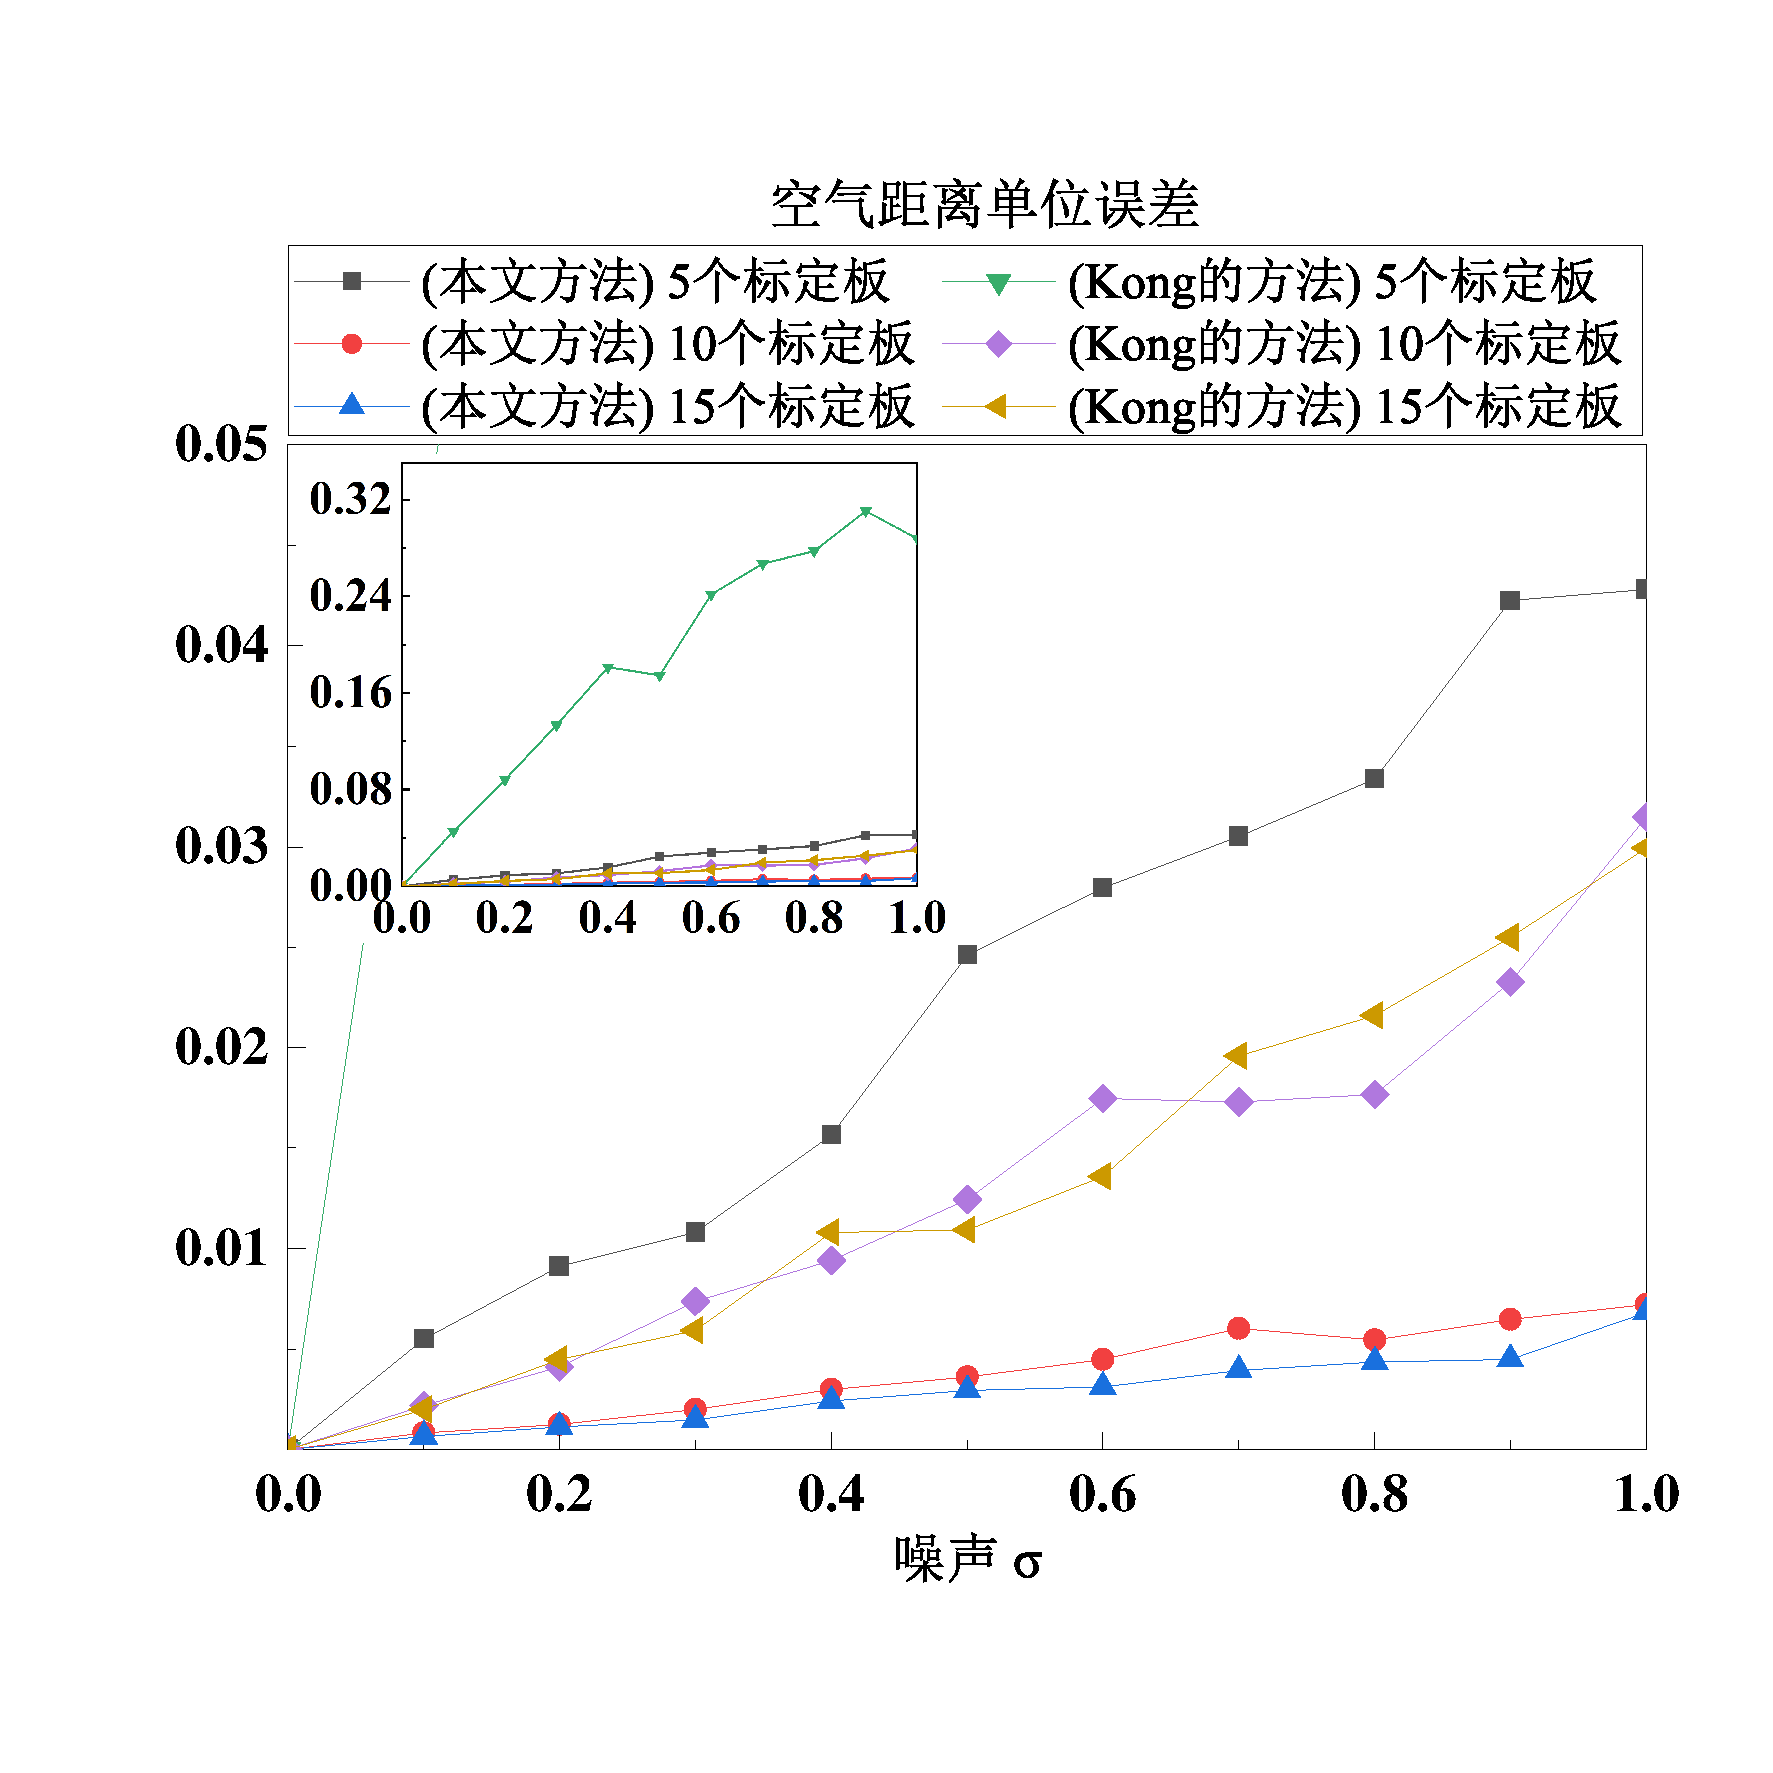
\includegraphics[width=7cm,height = 6.9cm]{毕设图片/2-4-1-1.pdf}}%
% %     \subfigure[{\fangsong 角度误差}] {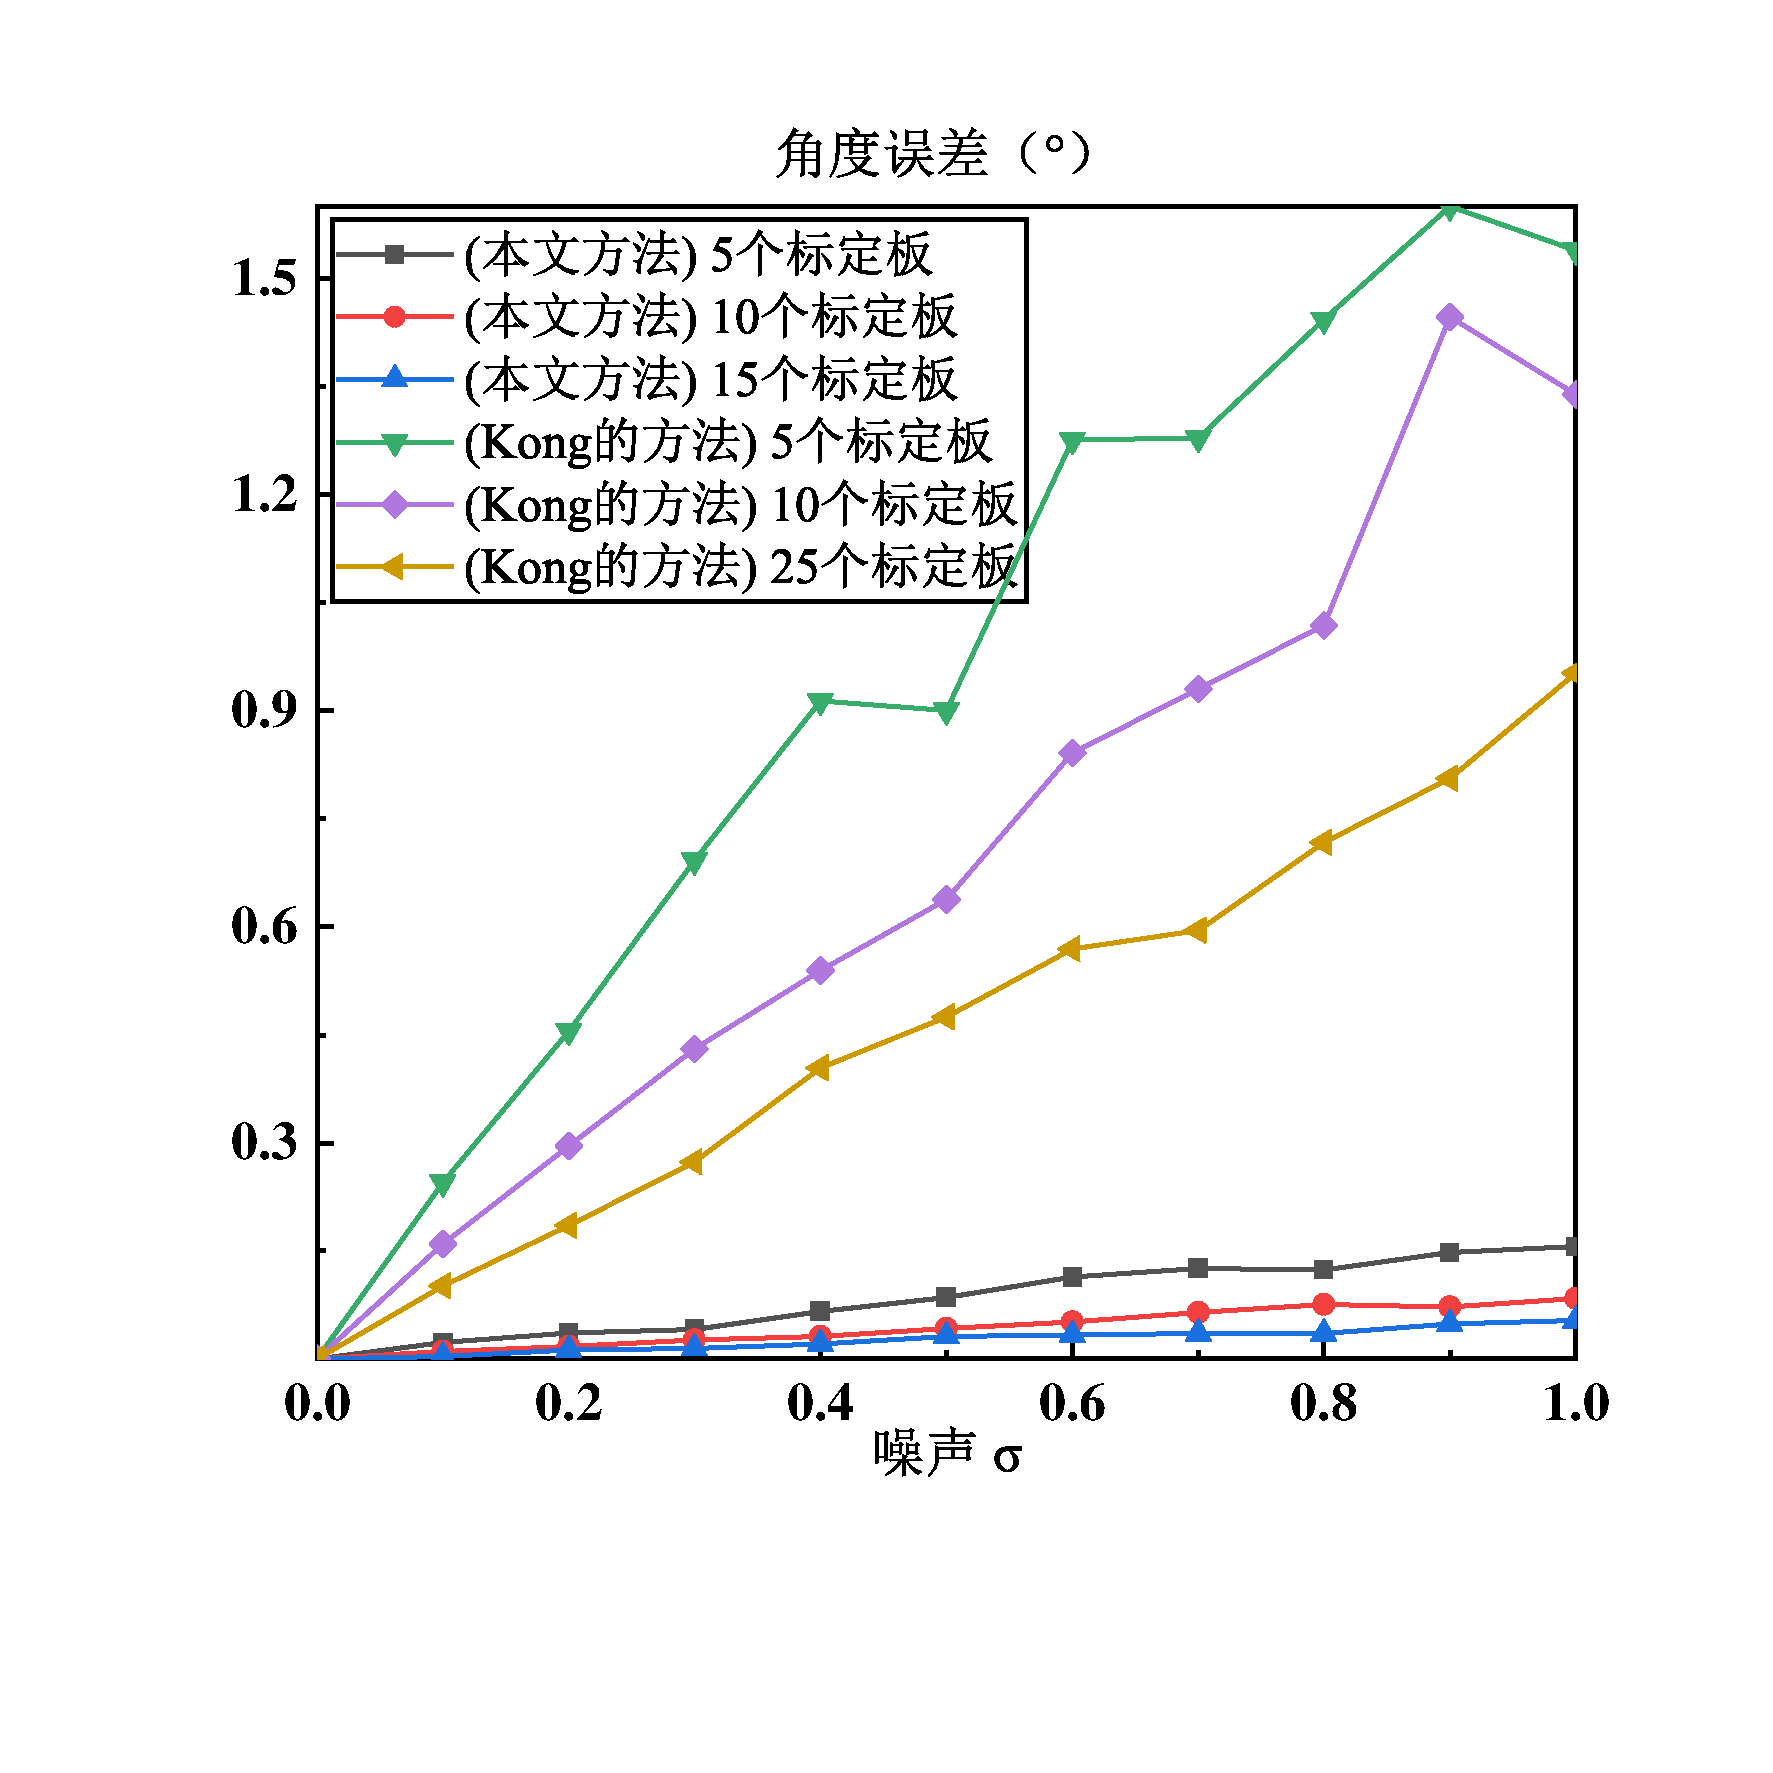
\includegraphics[width=7cm,height = 7cm]{毕设图片/2-4-2.pdf}}
% %     \subfigure[{\fangsong 重投影误差}] {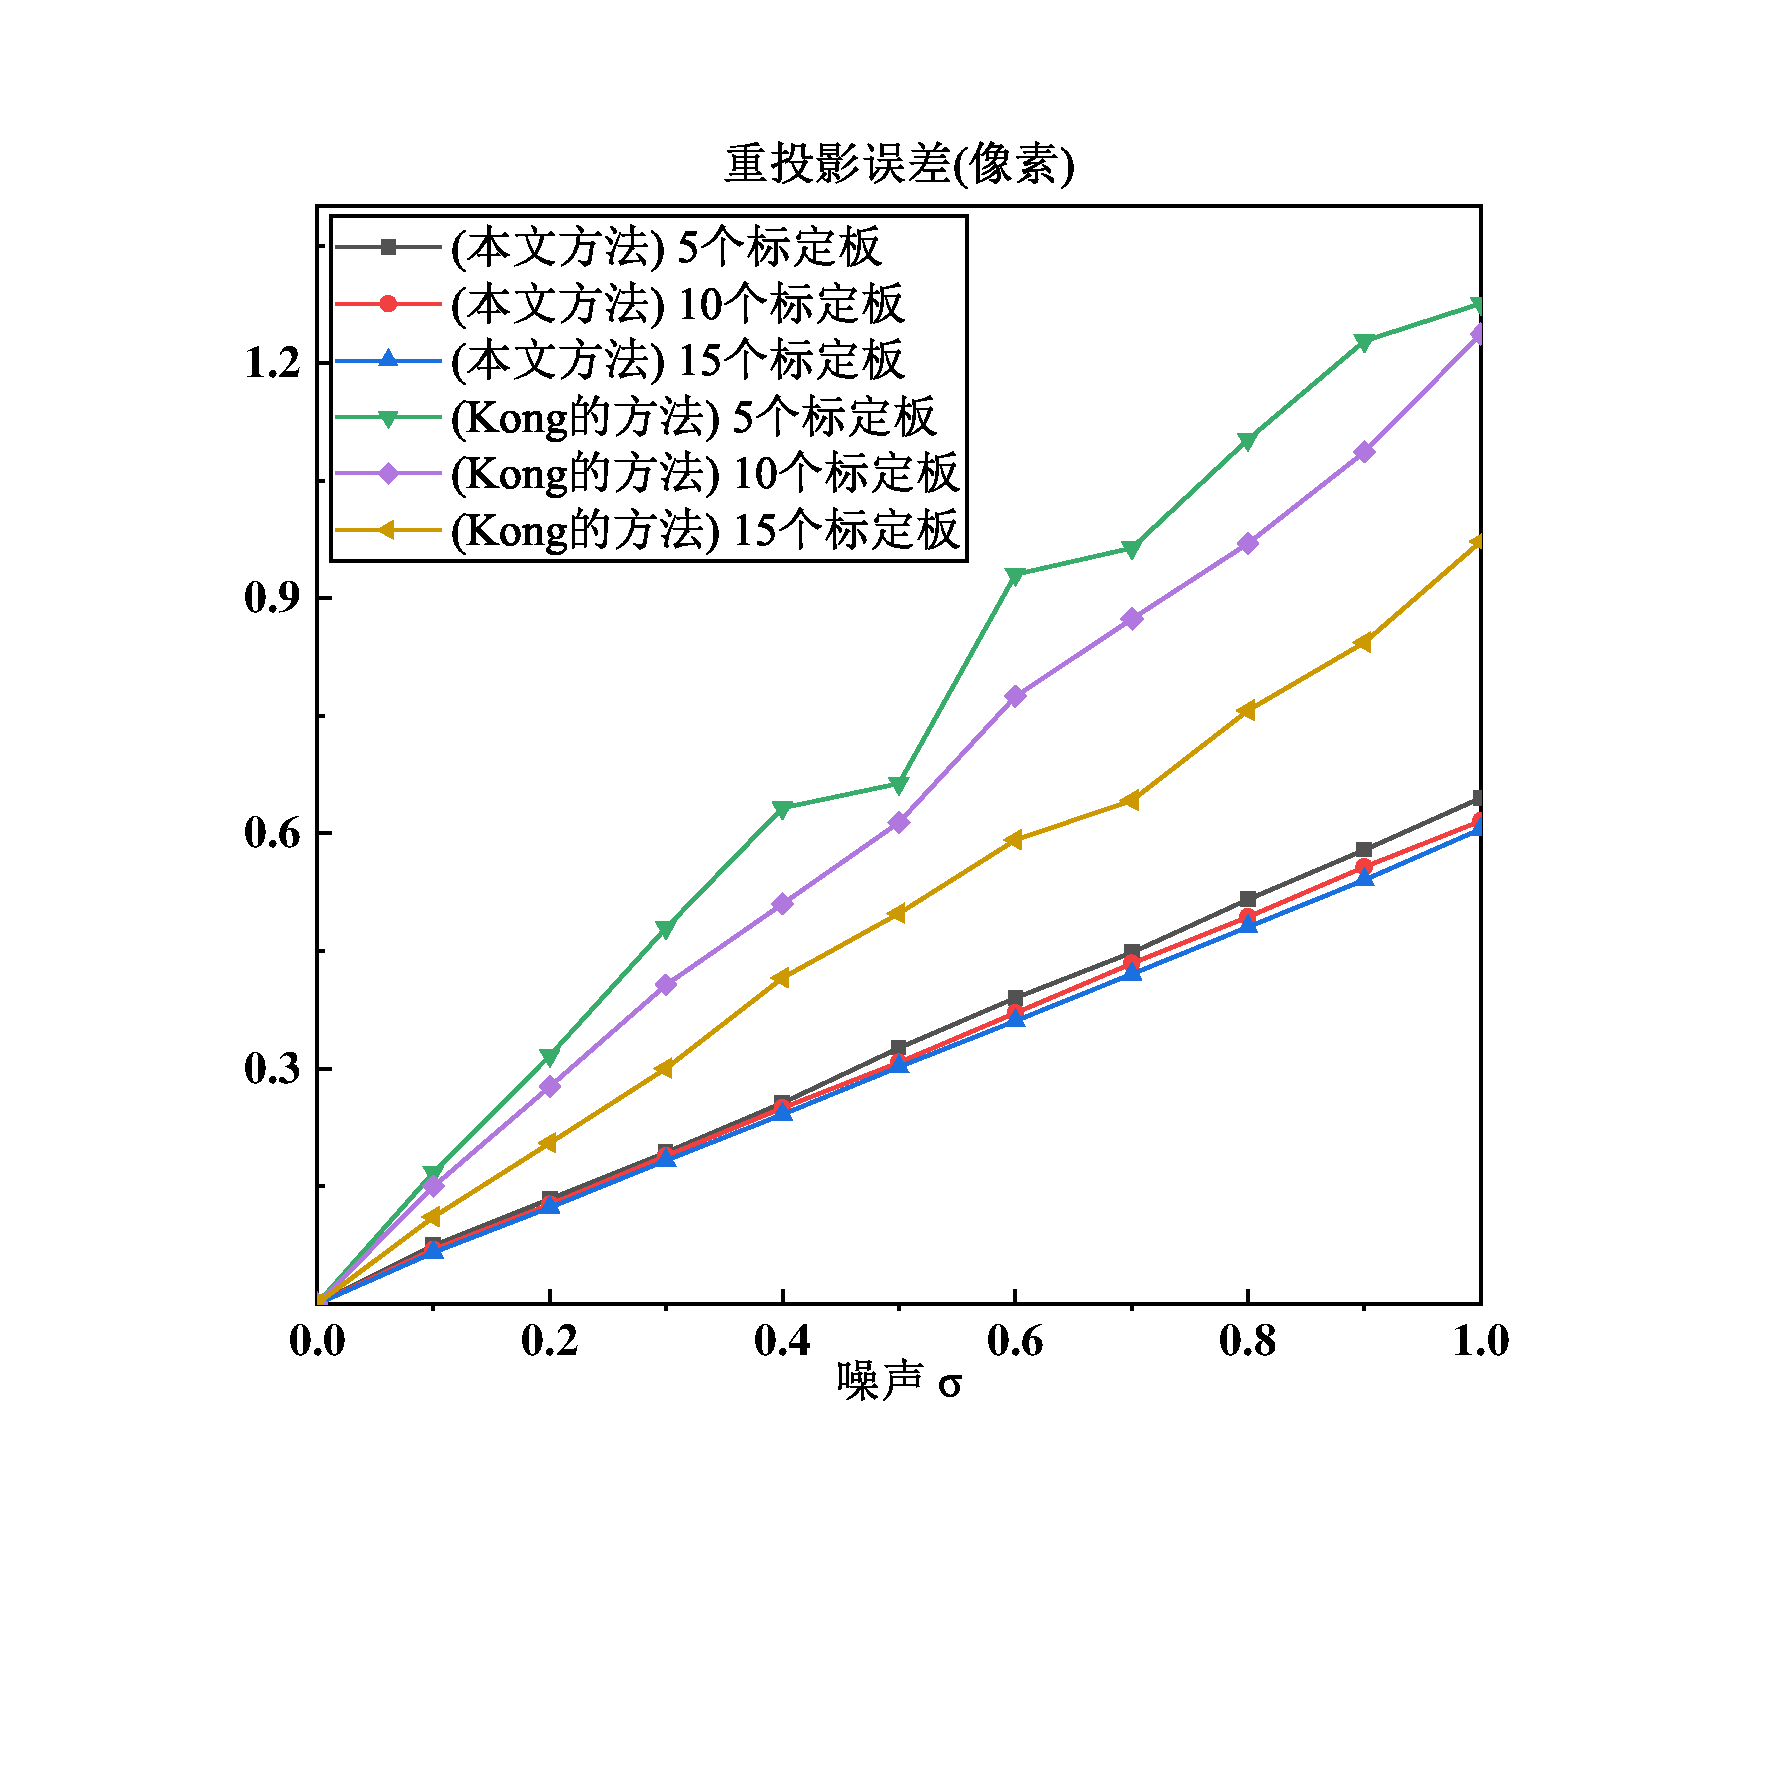
\includegraphics[width=7cm,height = 7cm]{毕设图片/2-4-3.pdf}}%
% %     \subfigure[{\fangsong 误差函数收敛情况}] {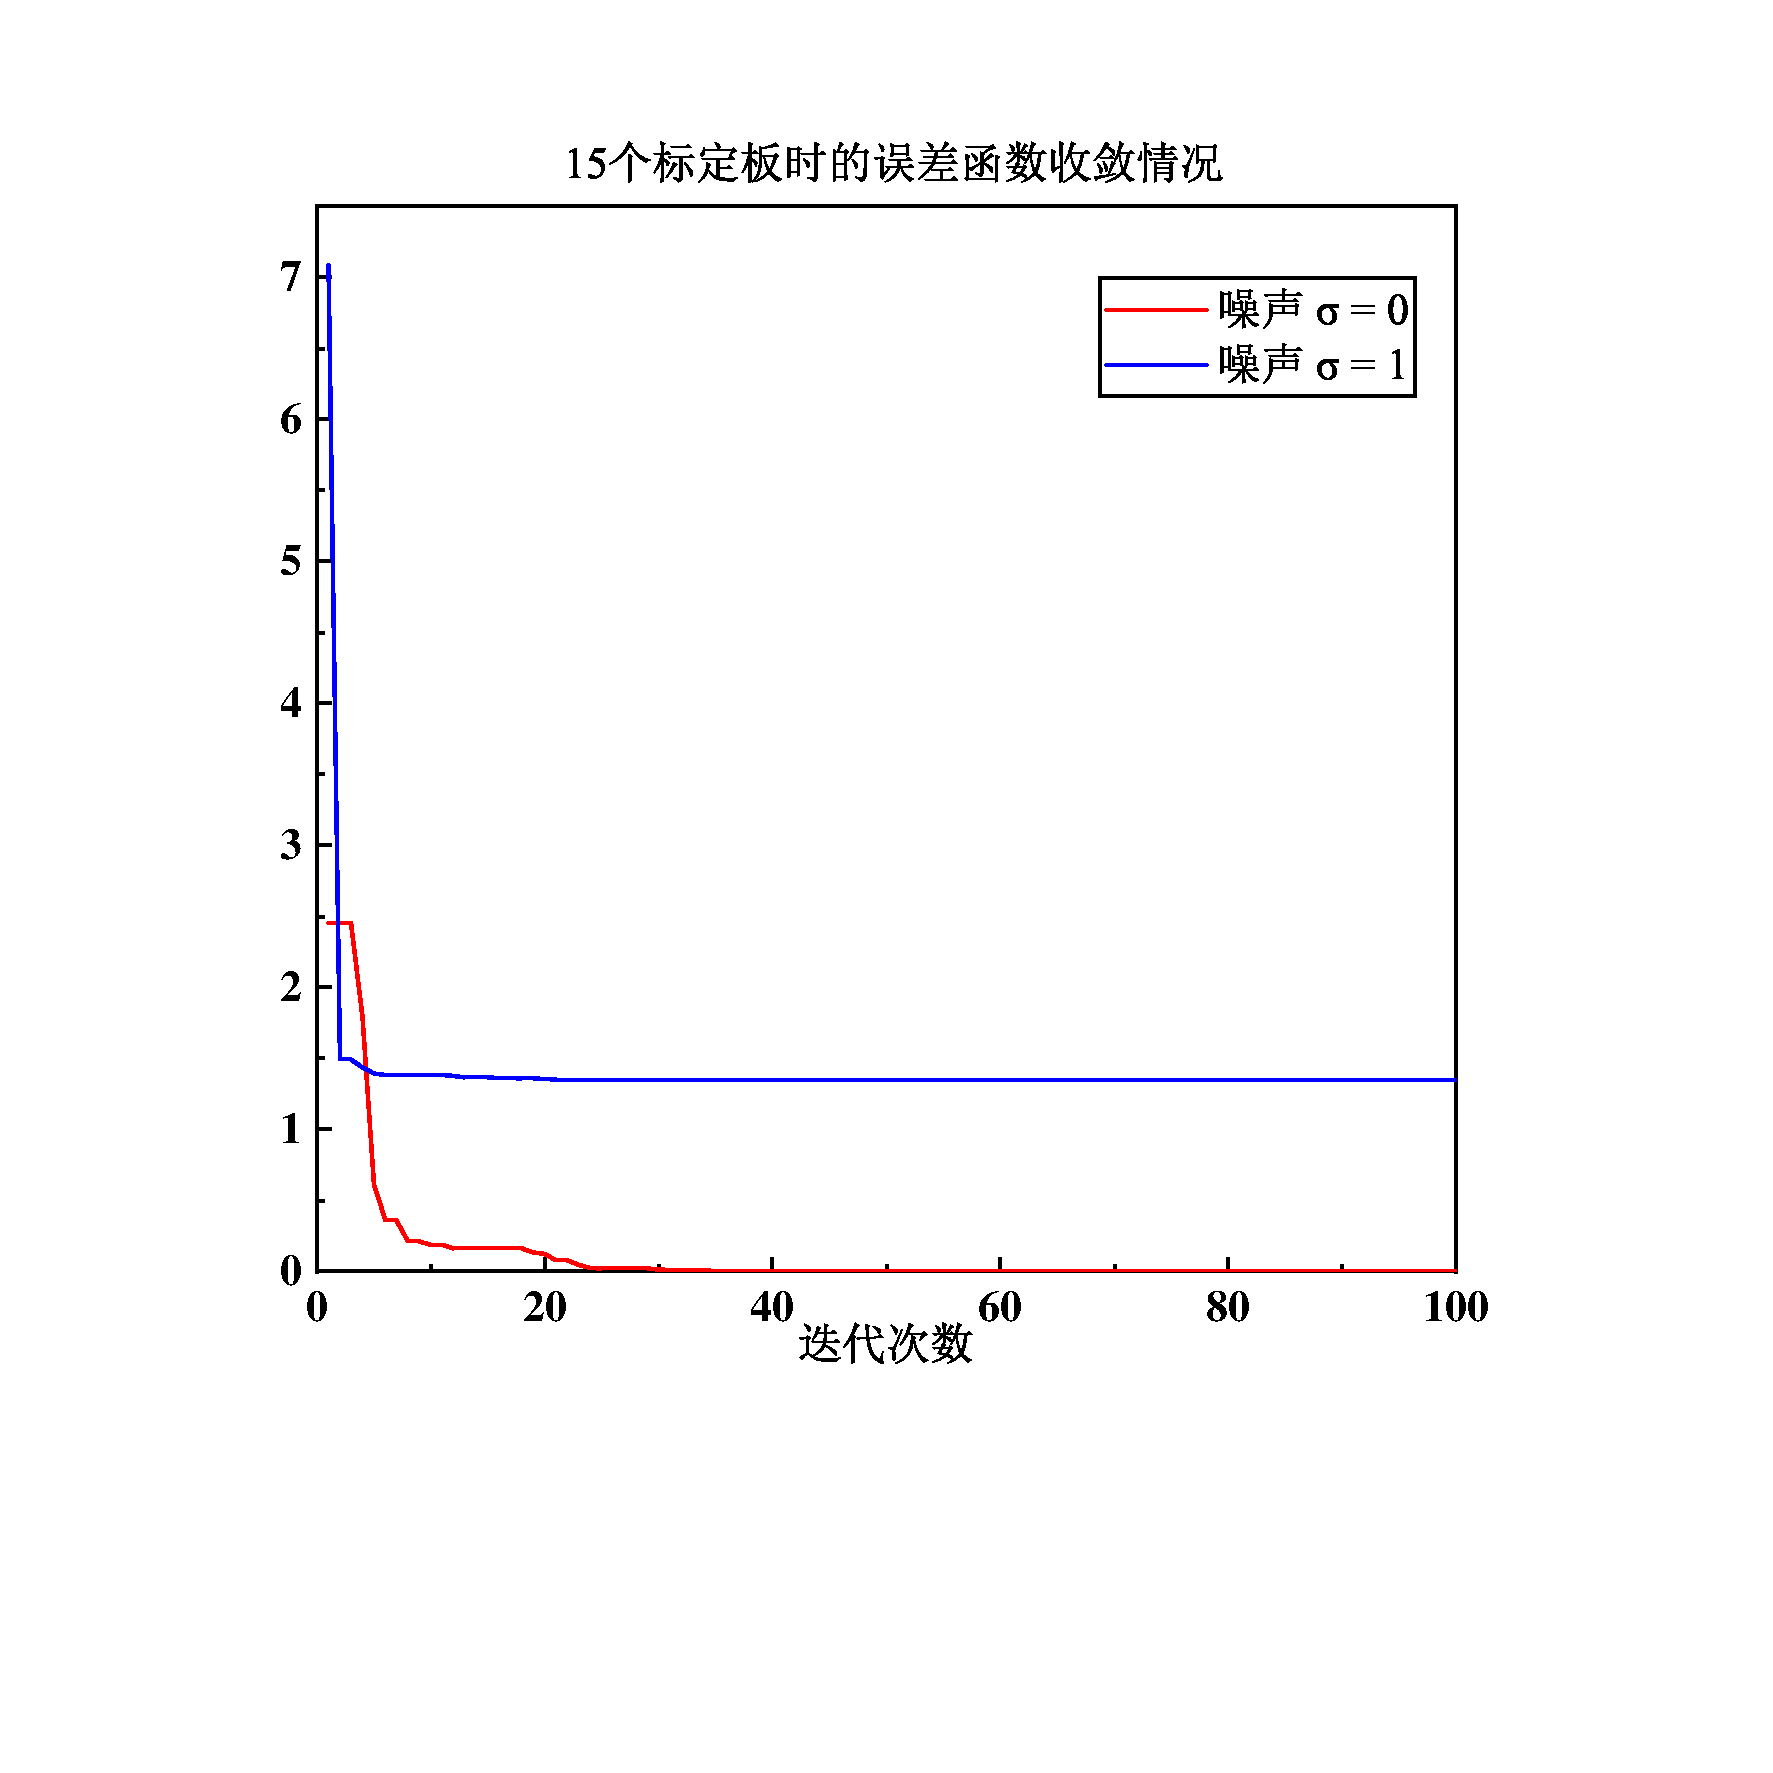
\includegraphics[width=7cm,height = 7cm]{毕设图片/2-4-4.pdf}}

% %     % 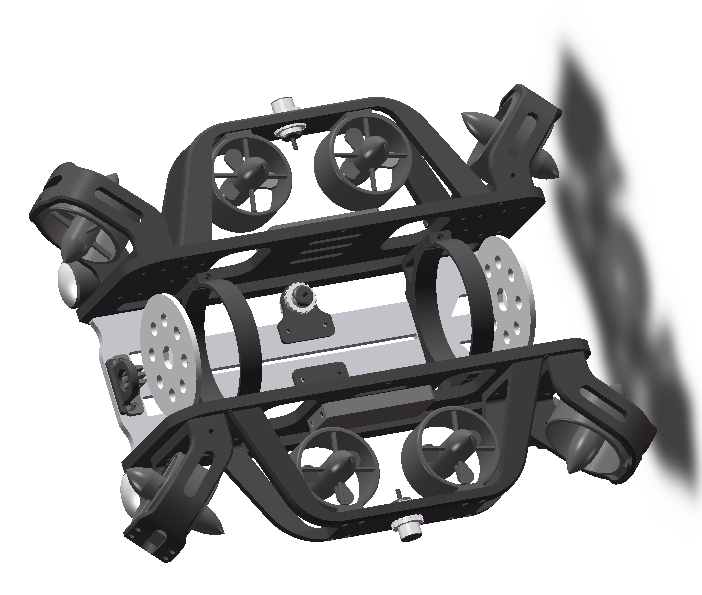
\includegraphics[width=14cm]{毕设图片/2-4}
% %     \caption{\label{fig:2-4}标定仿真结果}
% % \end{figure}



% \section{水下图像折射复原}
% 在完成水下双目的标定后,将水下双目相机图像进行极线矫正\cite{极线矫正}和立体匹配\cite{立体匹配} 。极线矫正通过改变相机内参和旋转平移矩阵能将左右相机的图像对齐,使得空间中的物体点投影到两个相机的像素点在同一像素纵坐标上。立体匹配通过构建左右相机视差损失函数,通过求解全局最小误差计算拍摄到的图像的视差图,找到个每一个空间点对应的右图中的像素坐标。使用前文获取到水下相机折射参数,通过2.3节中像素点与三维点的对应关系计算出图像上每一个像素点对应的空间点坐标,即每一帧图像的点云,再将空间点通过空气成像真空模型投影到像素平面上,即能得到没有水的场景下拍摄到的图。

% \subsection{极线矫正}
% 在完成了双目相机的内外参数标定后,能获取两个相机的刚体变换矩阵,但由于相机位置和角度的变化,同一实体在两幅图像中的位置可能不同,会导致视差在$x$方向和$y$方向均存在。如\autoref{fig:2-5}所示,双目相机在立体矫正前两个相机光芯是不平行的,极线矫正可以通过将图像进行适当的变换,使得两幅图像的光轴平行,且其中相应的特征点在同一水平线上,即$y$坐标相同,这样可以简化立体匹配的问题。
% \begin{figure}[htbp]
%     \centering
%     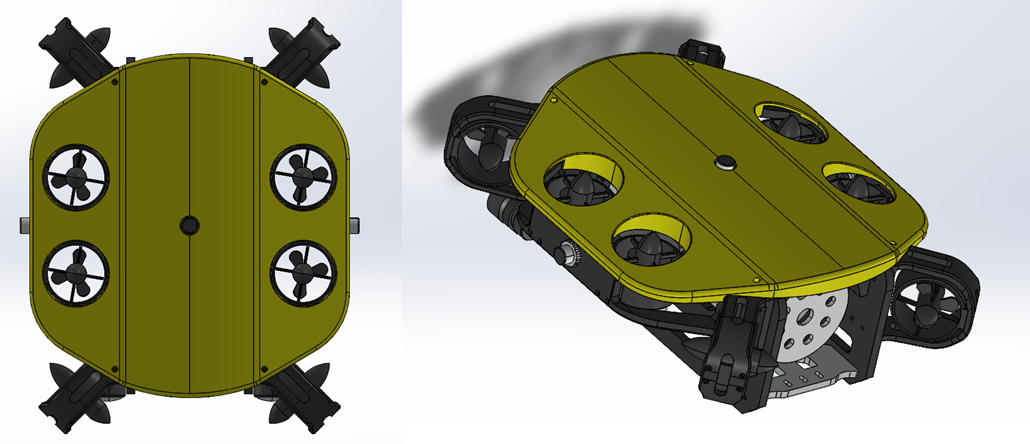
\includegraphics[width=14.5cm]{毕设图片/2-5}
%     \caption{\label{fig:2-5}立体矫正效果}
% \end{figure}

% 为了完成\autoref{fig:2-5}中的变换,本文采用的方法是左右相机成像平面各转一半,最后调整内参使得两个相机的光芯连线与成像平面平行。
% 通过双目标定能够得到两个相机的变换矩阵满足以下关系:
% \begin{equation}
%     \label{equ:2-27}
%     {{\bf{P}}_{l}} = {\bf{R}}{{\bf{P}}_{r}} + {\bf{t}}
% \end{equation}
% 其中${\bf{P}}_{l}$为左相机坐标系下的点,${\bf{P}}_{r}$为右相机坐标系下的点。
% 记{\bf{R}}矩阵旋转一半时的矩阵为{\bf{r}},则使得左相机的点变换为${{\bf{P}}_l}^\prime  = {{\bf{r}}^{-1}}{{\bf{P}}_l}$,右相机的点变换为${{\bf{P}}_r}^\prime  = {\bf{r}}{{\bf{P}}_r}$,使得两个相机成像平面平行。

% 为了使光芯连线与成像平面平行,首先计算平移矩阵{\bf{t}}与$x$轴的旋转轴,${\bf{w}} = {\bf{t}} \times {\left[ {\begin{array}{*{20}{c}}
%     1&0&0
%     \end{array}} \right]^T}$,旋转角为平移向量与$x$轴的夹角,即:
% \begin{equation}
%     \label{equ:2-27}
%     \alpha  = \arccos \left( {{{{\bf{t}} \cdot {{\left[ {\begin{array}{*{20}{c}}
%         0&0&1
%         \end{array}} \right]}^T}} \mathord{\left/
%          {\vphantom {{{\bf{t}} \cdot {{\left[ {\begin{array}{*{20}{c}}
%         0&0&1
%         \end{array}} \right]}^T}} {\left| {\bf{t}} \right|}}} \right.
%          \kern-\nulldelimiterspace} {\left| {\bf{t}} \right|}}} \right)
% \end{equation}
% 记旋转轴{\bf{w}}与旋转角$\alpha$组成的旋转矩阵为${{\bf{R}}_w}$,对左右相机都旋转${{\bf{R}}_w}$有
% \begin{equation}
%     \label{equ:2-28}
%     {{\bf{P}}_l}^{\prime \prime } = {{\bf{R}}_w}{{\bf{P}}_l}^\prime 
% \end{equation}
% \begin{equation}
%     \label{equ:2-28}
%     {{\bf{P}}_r}^{\prime \prime } = {{\bf{R}}_w}{{\bf{P}}_r}^\prime 
% \end{equation}

% 为了使两个相机图像在$y$轴平齐,下面调整内参,使得两个相机内参相等,令焦距为两个相机的焦距的平均值
% \begin{equation}
%     \label{equ:2-28}
%     {f_x} = {f_y} = \left( {{f_{yl}} + {f_{yr}}} \right)/2
% \end{equation}
% 并取相机主点${c_x}$、${c_y}$为分辨率值的一半,这样可使得主点在中心。

% \autoref{fig:2-6}和\autoref{fig:2-7}为本文在试验中测试的立体矫正的效果,本文绘制了红色水平线便于观察两个图像中同一目标的高度偏移;特别的,在立体矫正前,白线连接的左右棋盘格角点不在一个纵坐标上,而在立体矫正后基本位于同一纵坐标上。
% \begin{figure}[H]
%     \centering
%     \includegraphics[width=14.5cm]{毕设图片/未立体矫正.png}
%     \caption{\label{fig:2-6}未立体矫正的水下图像}
% \end{figure}

% \begin{figure}[H]
%     \centering
%     \includegraphics[width=14.5cm]{毕设图片/立体矫正.png}
%     \caption{\label{fig:2-7}立体矫正后的水下图像}
% \end{figure}



% \subsection{立体匹配}

% 在完成图像的极线矫正后,对图像进行立体匹配计算视差图。在极线矫正后,一般认为左右图像上相同点的纵像素坐标是相同的。因此,立体匹配是计算同一空间点在右图中的$x$坐标与左图中的$x$坐标的差值。

% 由于本文专注于水下三维重建,并不研究立体匹配算法,本文直接使用现有的立体匹配算法——ZED SDK立体匹配算法。\autoref{fig:2-8}是使用上一节立体矫正后的标定板所计算的视差图可视化结果,其中暖色代表值大,冷色代表值小。

% \begin{figure}[htbp]
%     \centering
%     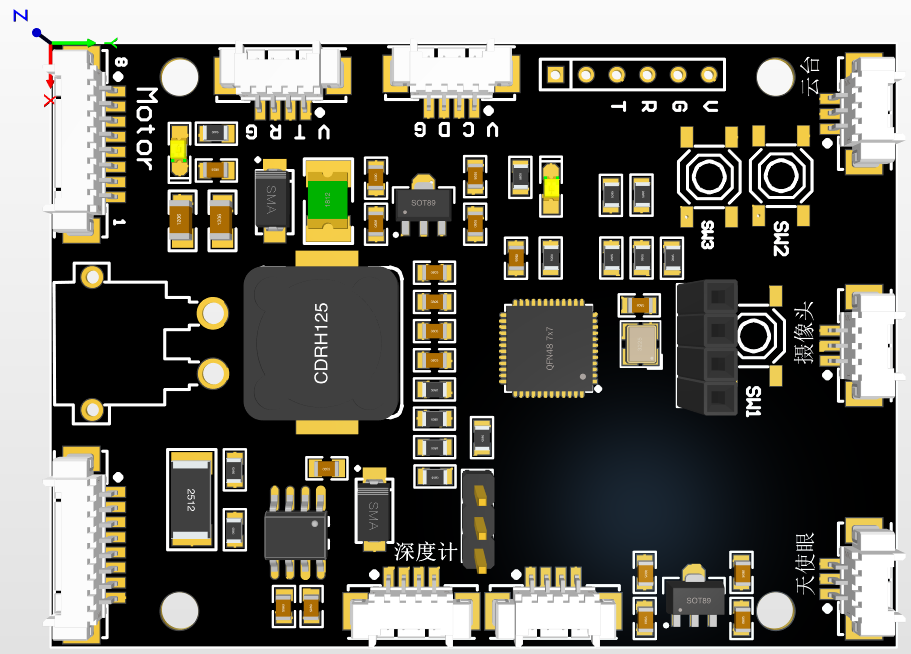
\includegraphics[width=10cm]{毕设图片/2-8.png}
%     \caption{\label{fig:2-8}立体匹配视差图可视化}
% \end{figure}

% \subsection{折射复原}

% 在完成水下相机标定和图像的立体匹配后,本节将使用视差图计算水中的三维点和折射复原彩色图像和深度图图像。
% 记左图为${I_l}$,视差图为${I_{dis}}$,矫正后左图对应的彩色图为${I_{rec}}$,矫正后左图对应的深度图为${I_{dep}}$,并用$\left( {i,j} \right)$表示这幅图像中第$i$行第$j$列的像素值。
% 通过2.3节中水下成像建模公式,可直接计算出左图像素点${I_l}\left( {i,j} \right)$对应的水中光线的向量${{\bf{v''}}_l}$,通过视差图能够得到该像素在右图中对应的像素坐标为$\left( {i,j - {I_{dis}}\left( {i,j} \right)} \right)$,将这个坐标同样代入2.3节的公式计算出水中的光线向量${{\bf{v''}}_r}$。最后使用2.3中的式 \eqref{equ:2-15}计算出这一点对应的三维点坐标,并使用针孔模型式 \eqref{equ:2-1}投影回像素平面,即可得到正确的RGB值,其深度图的值为这一点的Z坐标。\autoref{fig:2-9}为使用前文所述的视差图和水下图像计算出的复原图,本文将在试验章节使用特征点匹配的方式验证算法的正确性。
% \begin{figure}[H]
%     \centering
%     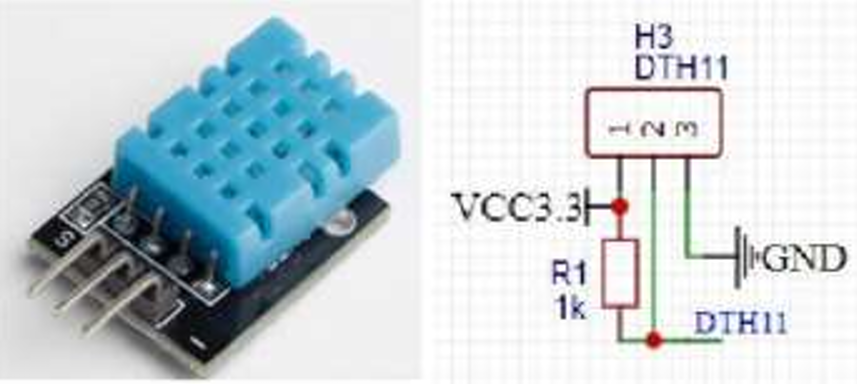
\includegraphics[width=14.5cm]{毕设图片/2-9}
%     \caption{\label{fig:2-9}折射复原结果}
% \end{figure}

% \subsection{GPU并行计算加速}
% 本章所提出的算法是为了能在水下SLAM系统中使用,SLAM系统通常运行帧率在30FPS以上,而在测试中发现在CPU上该算法难以达到SLAM系统要求的实时性,所以本节将使用GPU(Graphics Processing Unit)对算法进行加速。
% 而本算法在计算复原图像时,对每一个像素点都是单独处理的,这也为GPU加速创造了条件。


% 本模块基于NVIDIA的GPU计算库CUDA开发,用于在GPU上运行的函数成为核函数。如\autoref{fig:2-10}所示,kernel在GPU上执行时会同时启动很多线程,一个核函数所启动的所有线程称为一个网格(grid),同一个网格上的线程共享相同的全局内存空间,grid是线程结构的第一层,而grid又可以分为很多线程块(block),一个线程块里面包含很多线程。算法\ref{alg:1}为图像复原算法的GPU实现方法,其中,由于相机在标定好后像素点对应的水中向量和角点坐标是固定的,为了提高效率可生成对应表格用于查找。

% \begin{figure}[H]
%     \centering
%     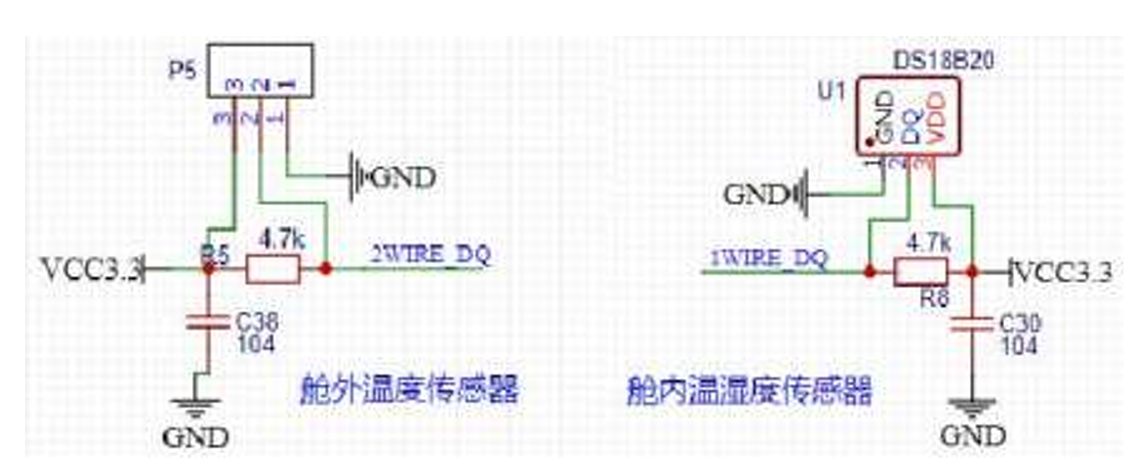
\includegraphics[width=10cm]{毕设图片/2-10}
%     \caption{\label{fig:2-10}核函数运行解析}
% \end{figure}

% 算法测试平台配置如下,CPU为Intel i5-10400F,GPU为NVIDIA RTX2060,内存条为16G。在CPU和GPU上运行效率如\autoref{tab:3},可见在GPU上运行帧率为142.9FPS,能够达到实时性。

% \begin{algorithm}[H]
%     % \renewcommand{\thealgocf}{3}     %<---细节与重点
%     \label{alg:1}
%     \fangsong
%     \SetAlgoLined
%     \KwIn{标定参数para,查找表Table,相机左图彩色图IR,相机左图视差图Dis}
   
%     \KwOut{左图折射复原图IRec,左图折射复原深度图IDRec}
    
% GPU执行参数:block.x = 32,block.y = 8\\
% \qquad \quad \qquad \qquad grid.x = (Image.width + 32 - 1)/32\\
% \qquad \quad \qquad \qquad grid.y = (Image.height + 32 - 1)/8

% KERNEL\_FUNCTION${\left \langle \left \langle \left \langle grid, block \right \rangle  \right \rangle  \right \rangle}$ (IR, Dis, para)

% KERNEL\_FUNCTION BEGIN:

% x = blockIdx.x * blockDim.x + threadIdx.x  // 像素横坐标

% y = blockIdx.y * blockDim.y + threadIdx.y  // 像素纵坐标

% Lp = Table(y, x)                        // 相机左图对应的水中的光线和坐标

% disU = x - Dis(y, x)                     // 相机左图中像素点对应的右图中的向量坐标

% rayR = ((disU - cx)/fx, (y - cy)/fy, 1)       // 相机右图像素点的归一化坐标

% 代入2.3节中的公式计算右图的像素点对应的光线和玻璃板表面的坐标Rp

% 代入2.3节中的公式计算水中交点point

% newU = fx * point.x / point.z + cx

% newV = fy * point.y / point.z + cy

% // 保存到IRec和IDRec共享内存中

% IRec.ptr(newV)[newU] = IR.ptr(y)[x]

% IDRec.ptr(newV)[newU] = point.z

% KERNEL\_FUNCTION END
 
% \caption{使用GPU加速的水下图像复原算法}
% \end{algorithm}



% %经典三线表
% \begin{table}[H]
%     \fangsong
%     \caption{\label{tab:3}折射复原算法效率对比}
%     \small %此处写字体大小控制命令
%     \centering%把表居中
%     \renewcommand{\arraystretch}{1.5}
%     \setlength{\tabcolsep}{8mm}{
%     \begin{tabular}{ccc}
%     \toprule%第一道横线
%     设备 & CPU & GPU    \\ 
%     \midrule%第二道横线 
%     每帧运行时间  & 73ms & 7ms              \\
%     帧率  & 13.7FPS & 142.9FPS                     \\
%     \bottomrule%第三道横线
%     \end{tabular}}
%     \end{table}
% \section{本章小结}

% 本章针对水下三维重建中的图像折射问题,构建了水下双目相机折射成像模型,并提出了标定算法,最后对图像进行折射复原处理。本章使用仿真对比了本文算法与Kong算法,证明了本章提出的算法在精度和鲁棒性上具有优势。此外,本章基于所标定的参数提出了水下图像折射复原算法,结合视差图计算出水下目标的点云,并反投影回像素坐标系计算出图像,最后使用GPU对算法进行加速,为后续的水下高精度视觉SLAM提供了基础。